\documentclass[a4paper,11pt,oneside]{book}

%%% το αρχείο αυτό καθορίζει το look που έχουν οι pythonies
%%% γίνεται \input από όλα τα κεφάλαια και τα φύλλα εργασίας

% χρησιμοποιούμενα πακέτα: 
% 
% polyglossia
% xstring
% graphicx
% caption
% xcolor
% hyperref
% minted
% geometry
% titlesec
% datetime
% changepage
% ntheorem

% οριζόμενες εντολές:
%
% smallcaps (βοηθ. removeaccents)
%    μικρά κεφαλαία χωρίς τόνους στα φωνήεντα
% scaling
%    η κλιμάκωση *όλων* των illustrations, τρέχουσα τιμή 0.9
% iconcomputer, iconkeyboard, icondiscuss, iconfillin, iconcaution, iconprompt, dottedline
%    εικονίδια για τα φύλλα εργασίας και εστιγμένη γραμμή
% marginnote
%    πλευρικό σχόλιο
% chapterwabstract (βοηθ. abstract, boxcolor, chaptercolor, concepts, tmpconcepts)
%    εισαγωγικό κείμενο κεφαλαίου με χρωματιστό τετράγωνο, συνοδευτικές έννοιες, κλπ.
% tobecontinued
%    εμφανίζει το "συνεχίζεται στην επόμενη σελίδα"

% οριζόμενα περιβάλλοντα:
% 
% note
%    μια υποσημείωση ή υπόδειξη, με μικρότερα γράμματα
% question
%    μια ερώτηση που "οδηγεί" κάθε νέα ενότητα
% answer
%    μια απάντηση σε μια ερώτηση του φύλλου εργασίας
% theory
%    μια ενότητα "θεωρίας" (στο τέλος ενός κεφαλαίου)
% exercise
%    μια αριθμημένη άσκηση
% step
%    ένα αριθμημένο βήμα (για φύλλο εργασίας)

% για μορφοποίηση κώδικα:
%
% pycode (περιβάλλον)
%     κώδικας python χωρίς αρίθμηση
% pyfile (εντολή)
%     εισαγωγή κώδικα python από αρχείο
% pyfilenl (εντολή)
%     εισαγωγή κώδικα python από αρχείο χωρίς αρίθμηση γραμμών
% pyfilesrc (εντολή)
%    εισαγωγή κώδικα από αρχείο με link στο αρχείο
% pyinline (εντολή)
%     κώδικας python μέσα στη ροή του κειμένου
% pyplain (περιβάλλον, για τα φύλλα εργασίας)
%     κώδικας python χωρίς φόντο
% pynew (περιβάλλον, για τα φύλλα εργασίας)
%     κώδικας python με φόντο
% pyterm (περιβάλλον για τα φύλλα εργασίας)
%     η είσοδος του χρήστη ή τα περιεχόμενα της οθόνης
% pyhighlight (εντολή)
%    highlight κειμένου (χρησιμοποιείται για κώδικα μέσα σε pyplain)


%%% επιλογές γλώσσας και γραμματοσειρών για το XeLaTeX

\usepackage{polyglossia}
\setdefaultlanguage{greek}
\setmainfont[Ligatures=TeX,SmallCapsFont={Linux Libertine O C},SmallCapsFeatures={Letters=SmallCaps}]{Linux Libertine O}
\setsansfont{Linux Biolinum O}
\setmonofont{Ubuntu Mono}
\enablehyphenation

% αφαίρεση τόνων από τα smallcaps
\usepackage{xstring}
\newcommand{\removeaccents}[1]{%
\def\result{#1}%
\StrSubstitute{\result}{ά}{α}[\result]%
\StrSubstitute{\result}{έ}{ε}[\result]%
\StrSubstitute{\result}{ή}{η}[\result]%
\StrSubstitute{\result}{ί}{ι}[\result]%
\StrSubstitute{\result}{ό}{ο}[\result]%
\StrSubstitute{\result}{ύ}{υ}[\result]%
\StrSubstitute{\result}{ώ}{ω}[\result]%
\StrSubstitute{\result}{Ά}{Α}[\result]%
\StrSubstitute{\result}{Έ}{Ε}[\result]%
\StrSubstitute{\result}{Ή}{Η}[\result]%
\StrSubstitute{\result}{Ί}{Ι}[\result]%
\StrSubstitute{\result}{Ό}{Ο}[\result]%
\StrSubstitute{\result}{Ύ}{Υ}[\result]%
\StrSubstitute{\result}{Ώ}{Ω}[\result]%
\result
}

\newcommand{\smallcaps}[1]{\textsc{\removeaccents{#1}}}

%%% εικόνες και λεζάντες

\usepackage{graphicx}
\newcommand{\scaling}{0.9}
\usepackage{caption}
\captionsetup{font=footnotesize}

%%% ειδικά περιβάλλοντα

\usepackage{xcolor}

% ερωτήσεις (που οδηγούν στην επόμενη ενότητα)
\definecolor{questioncolor}{rgb}{0.6,0.5,0.5}
\newenvironment{question}{\noindent\itshape\color{questioncolor}}{\noindent\ignorespaces}

% απαντήσεις (για τις ερωτήσεις των φύλλων εργασίας)
\definecolor{answercolor}{rgb}{0.5,0.5,0.5}
\newenvironment{answer}{\marginnote[16pt]{\iconfillin}\noindent\itshape\color{answercolor}}{\noindent\ignorespaces}

% περιβάλλον "θεωρίας" (πλήρες πλάτος κειμένου)
\usepackage{changepage}
\newenvironment{theory}[1]{\begin{adjustwidth}{}{-\overhang}\smallcaps{#1}\itshape}{\end{adjustwidth}}

% απομεινάρια...
% \newlength{\theoryrulelength}
% \setlength{\theoryrulelength}{36pt}
% \newenvironment{theory}{\rule{\theoryrulelength}{0.4pt}\begin{adjustwidth}{}{-\overhang}\itshape}{\end{adjustwidth}\rule{\theoryrulelength}{0.4pt}}

%%% υπερσύνδεσμοι

\definecolor{linkcolor}{rgb}{0.0,0.5,0.25}
\usepackage[colorlinks=true,urlcolor=linkcolor]{hyperref}

%%% εικονίδια και εστιγμένες γραμμές (για τα φύλλα εργασίας)

\newcommand{\iconcomputer}{
\includegraphics[scale=0.35]{../../share/circle-icons/one-color/computer.eps}}
\newcommand{\iconkeyboard}{
\includegraphics[scale=0.35]{../../share/circle-icons/one-color/keyboard.eps}}
\newcommand{\icondiscuss}{
\includegraphics[scale=0.35]{../../share/circle-icons/one-color/chat.eps}}
\newcommand{\iconfillin}{
\includegraphics[scale=0.35]{../../share/circle-icons/one-color/compose.eps}}
\newcommand{\iconcaution}{
\includegraphics[scale=0.35]{../../share/circle-icons/one-color/caution.eps}}
\newcommand{\iconprompt}{
\includegraphics[scale=0.35]{../../share/circle-icons/one-color/prompt.eps}}
\newcommand{\dottedline}{\vspace{\parskip}\dotfill}

%%% συνεχίζεται στην επόμενη σελίδα

\newcommand{\tobecontinued}{\mbox{}\hfill{\footnotesize ...συνεχίζεται στην επόμενη σελίδα.}}
\newenvironment{note}{\small\upshape}{}

%%% μορφοποίηση κώδικα με το pygmentize

\usepackage{minted}

% fix για ένα bug στο minted που εμφανίζεται όταν χρησιμοποιείται χρώμα στο φόντο (bgcolor)
% http://tex.stackexchange.com/questions/228058/how-to-space-before-and-after-a-minted-code-block-with-bgcolor
\makeatletter
\patchcmd{\minted@colorbg}{\noindent}{\noindent}{}{}
\apptocmd{\endminted@colorbg}{}{}{}
\makeatother

% χρώματα φόντου για τον κώδικα
\definecolor{codebg}{rgb}{0.80,0.95,0.85}
\definecolor{newcodebg}{rgb}{0.75,0.95,0.85}

% ορισμοί για τα περιβάλλοντα κώδικα
% pycode: περιβάλλον κώδικα python χωρίς αρίθμηση
\newminted[pycode]{python3}{bgcolor=codebg}
% pyfile: python από αρχείο
\newmintedfile[pyfile]{python3}{linenos=true,numberblanklines=false,escapeinside=||,bgcolor=codebg}
% pyfilenl: python από αρχείο χωρίς αρίθμηση γραμμών
\newmintedfile[pyfilenl]{python3}{linenos=false,numberblanklines=false,escapeinside=||,bgcolor=codebg}
% pyinline: python μέσα στη ροή του κειμένου
\newmintinline[pyinline]{python3}{linenos=true,numberblanklines=false}
% pyplain: (για τα φύλλα εργασίας) περιβάλλον χωρίς φόντο
\newminted[pyplain]{python3}{bgcolor=white,escapeinside=||,formatcom={\upshape}}
% pynew: (για τα φύλλα εργασίας) περιβάλλον με φόντο
\newminted[pynew]{python3}{bgcolor=newcodebg,escapeinside=||,formatcom={\upshape}}
% pyterm: (για τα φύλλα εργασίας) περιβάλλον για τα περιεχόμενα της οθόνης
\newminted[pyterm]{text}{bgcolor=white,escapeinside=||}

%\newminted[pyterm]{text}{escapeinside=||}
% [TODO] fix: το pyterm χωρίς bgcolor εμφανίζει μεγαλύτερα περιθώρια (πάνω και κάτω) και δεν φαίνεται ωραίο. Το bgcolor είναι προσωρινό workaround, έχει κι αυτό margins (για να μην είναι κολλητά ο κώδικας με το περιθώριο) κι έτσι ο κώδικας στ' αριστερά δεν είναι τέλεια στοιχισμένος.

% εντολή για κώδικα από αρχείο με link στο αρχείο
\newcommand{\pyfilesrc}[2][]{%
\pyfile[#1]{#2}\\
\mbox{}\hfill{\scriptsize\href{http://pythonies.mysch.gr/#2}{\url{#2}}}
}

% εντολή για το highlighting του κώδικα (συνήθως σε pyplain περιβάλλον με escapeinside)
\newcommand{\pyhighlight}[1]{\colorbox{newcodebg}{#1}}

%%% αριθμημένα περιβάλλοντα

\usepackage{ntheorem}

% άσκηση
\makeatletter
\theoremheaderfont{\upshape}%\upshape\bfseries\scshape}
\theorembodyfont{\itshape}%\slshape}
\newtheoremstyle{lmargin}%
  {\item[\theorem@headerfont \llap{##2}\hskip\labelsep\hskip-6pt]}%
  {\item[\theorem@headerfont \llap{##2}\hskip\labelsep ##1\ (##3)\theorem@separator]}
\makeatother
\theoremstyle{lmargin}
\newtheorem{exercise}{}[chapter]

% βήμα φύλλου εργασίας
\makeatletter
\theoremheaderfont{\bfseries}%\upshape\bfseries\scshape}
\theorembodyfont{\upshape}%\slshape}
\newtheoremstyle{lmarginup}%
  {\item[\theorem@headerfont \llap{##2}\hskip\labelsep\hskip-6pt]}%
  {\item[\theorem@headerfont \llap{##2}\hskip\labelsep ##1\ (##3)\theorem@separator]}
\newtheoremstyle{slmarginup}%
  {\item[\theorem@headerfont \llap{##1##2.}\hskip\labelsep\hskip-6pt]}%
  {\item[\theorem@headerfont \llap{##2.}\hskip\labelsep ##1\ (##3)\theorem@separator]}
\makeatother

% deprecated: \newcommand{\standalone}{} to define standalone
%\ifdefined\standalone
    \theoremstyle{slmarginup}
    \newtheorem{step}{}
%\else
%    \theoremstyle{lmarginup}
%    \newtheorem{step}{}[chapter]
%\fi

%%% γεωμετρία σελίδας και συναφείς ορισμοί από το tufte-latex
%%% https://tufte-latex.github.io/tufte-latex/

% εσοχή και διάστημα μεταξύ παραγράφων
% δεν επηρρεάζει το tufte-latex
\parindent=0pt
\parskip=6pt

% γεωμετρία σελίδας και ορισμός μηκών
\usepackage[a4paper,left=24.8mm,top=27.4mm,headsep=2\baselineskip,textwidth=107mm,marginparsep=8.2mm,marginparwidth=49.4mm,textheight=66\baselineskip,headheight=\baselineskip]{geometry}

\setlength{\marginparpush}{12pt}
\addtolength{\marginparpush}{\parskip}
\newlength{\fullwidth}
\setlength{\fullwidth}{\textwidth}
\addtolength{\fullwidth}{\marginparsep}
\addtolength{\fullwidth}{\marginparwidth}
\newlength{\overhang}
\setlength{\overhang}{\marginparsep}
\addtolength{\overhang}{\marginparwidth}

% απομεινάρια...
%\setlength\abovedisplayskip{6pt plus 2pt minus 4pt}
%\setlength\belowdisplayskip{6pt plus 2pt minus 4pt}

% italicize description run-in headings (instead of the default bold)
\renewcommand*\descriptionlabel[1]{\hspace\labelsep\normalfont\em #1}

% πλευρική σημείωση
\newcommand\marginnote[2][0pt]{%
  \marginpar{\hbox{}\vspace*{#1}\vspace*{-1\baselineskip}\noindent \footnotesize\textup{#2}}%
  {}%
}

% formatting title sections
\setcounter{secnumdepth}{-1}

\usepackage{titlesec}
\usepackage[nodate]{datetime}
\newlength{\beforesection}
\setlength{\beforesection}{3ex plus 0.5ex minus 0.2ex}
\addtolength{\beforesection}{-\parskip}
\newlength{\aftersection}
\setlength{\aftersection}{1.5ex plus 0.2ex}
\addtolength{\aftersection}{-\parskip}
\titlespacing*{\section}{0pt}{\beforesection}{\aftersection}

% απομεινάρια...
%\titlespacing*{\chapter}{0pt}{50pt}{40pt}
%\titlespacing*{\section}{0pt}{3.5ex plus 1ex minus .2ex}{2.3ex plus .2ex}

%%% για εισαγωγικό κείμενο κεφαλαίου με χρωματιστό τετράγωνο, συνοδευτικές έννοιες, κλπ.

\newcommand{\abstract}{}
\newcommand{\boxcolor}{}
\newcommand{\chaptercolor}{}
\newcommand{\concepts}{}
\newcommand{\tmpconcepts}{}
\newif\ifbonus

% reference: \titleformat{ command }[ shape ]{ format }{ label }{ sep }{ before-code }[ after-code ]
\titleformat{\chapter}[block]
{\Huge\sffamily}
{}
{0pt}
{\ifbonus\marginnote[-6pt]{\fcolorbox{\boxcolor}{\chaptercolor}{\makebox(40,40){\strut\textcolor{\boxcolor}{\Huge\thechapter}}}\\\vspace{\parskip}\\\tiny\today\\ \currenttime}\else\marginnote[-6pt]{\colorbox{\boxcolor}{\makebox(40,40){\strut\textcolor{\chaptercolor}{\Huge\thechapter}}}\\\vspace{\parskip}\\\tiny\today\\ \currenttime}\fi}
[\small\rmfamily\textmd\abstract\vspace{\parskip}\concepts\vspace{\parskip}\\\mbox{}\hrulefill]

\newcommand{\chapterwabstract}[5]{
	\renewcommand{\abstract}{#2}
    \renewcommand{\tmpconcepts}{#3}
	\ifdefempty{\tmpconcepts}{\renewcommand{\concepts}{}}{\renewcommand{\concepts}{\\\textbf{Έννοιες: }\tmpconcepts}}
	\renewcommand{\boxcolor}{#4}
	\renewcommand{\chaptercolor}{#5}
	\chapter{#1}
}

\definecolor{introColor}{rgb}{0.25,0.5,0.75}
\definecolor{answerColor}{rgb}{0.25,0.75,0.5}
\definecolor{crapsColor}{rgb}{0.5,0.75,0.25}
\definecolor{subtractionColor}{rgb}{0.5,0.25,0.75}
\definecolor{guessColor}{rgb}{0.75,0.25,0.5}
\definecolor{nimColor}{rgb}{0.75,0.5,0.25}
\definecolor{planetColor}{rgb}{0.25,0.25,0.75}
\definecolor{hangmanColor}{rgb}{0.25,0.75,0.25}
\definecolor{oxoColor}{rgb}{0.75,0.25,0.25}

\setcounter{part}{2}
\setcounter{chapter}{5}

%%% DOCUMENT START

\begin{document}

\chapterwabstract{Διαπλανητικό Κουίζ}{Στο κεφάλαιο αυτό θα υλοποιήσουμε ένα παιχνίδι ερωτήσεων με θέμα τους πλανήτες του ηλιακού μας συστήματος. Ο παίκτης θα καλείται να βρει έναν πλανήτη από τη θέση του στο ηλιακό σύστημα, να τον μαντέψει από τους γειτονικούς του πλανήτες ή να βάλει τους πλανήτες σε σωστή σειρά,  Οι ερωτήσεις που θα τίθενται στον παίκτη δεν θα είναι οι ίδιες κάθε φορά, αλλά θα δημιουργούνται δυναμικά, κατά την εκτέλεση του προγράμματος. Μέσα από το πρόγραμμά μας θα γνωρίσουμε μια πολύ σημαντική έννοια στον προγραμματισμό, τη δομή δεδομένων και πιο συγκεκριμένα μια δομή δεδομένων που ονομάζεται λίστα. Θα έχουμε επίσης την ευκαιρία να εξοικειωθούμε ακόμη περισσότερο με τα υποπρογράμματα, μιας και όλο το πρόγραμμα υλοποιείται με τη βοήθειά τους.}{λίστες, υποπρογράμματα}{planetColor}{white}

% [comment] προσθήκη σχολίου: σκοπός μας δεν είναι η καλύτερη δυνατή υλοποίηση, αλλά η κατανόηση βασικών εννοιών για τις λίστες.

%%%%%%%%

% [TODO] VERY IMPORTANT: Να διαφοροποιείται με κάποιο τρόπο ο υπάρχων κώδικας, από τον καινούργιο που μπαίνει ή από τον κώδικα που βγαίνει.

\section{Όλοι οι Καλοί Χωράνε}

\begin{question}
Πού θα καταχωρίσω τα ονόματα όλων των πλανητών του ηλιακού συστήματος;
\end{question}

\marginnote[18pt]{
\begin{center}
    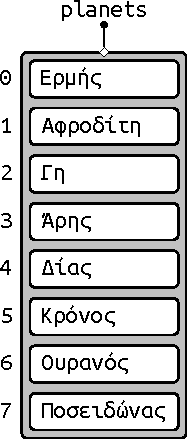
\includegraphics[scale=\scaling]{illustrations/planets.pdf}
    \captionof{figure}{Η λίστα με τα ονόματα των πλανητών. Οι θέσεις της λίστας είναι αριθμημένες. Με βάση τους αριθμούς των θέσεων μπορούμε ν' αναφερθούμε σε κάθε στοιχείο ξεχωριστά. Προσοχή όμως, η αρίθμηση \emph{ξεκινά από το 0}.}
\end{center}}
Για να μπορεί το πρόγραμμά μας να ``δημιουργεί'' ερωτήσεις προς τον χρήστη θα πρέπει να έχει διαθέσιμα τα ονόματα όλων των πλανητών. Μέχρι στιγμής
χρειάστηκε να αποθηκεύσουμε τιμές και να αναφερθούμε σε αυτές χρησιμοποιώντας μεταβλητές. Πολύ συχνά όμως χρειάζεται να αποθηκεύσουμε μια ομάδα τιμών με τη μορφή μιας \emph{συλλογής}. Με τον τρόπο αυτό θα έχουμε πρόσβαση σε όλα τα στοιχεία της ομάδας χρησιμοποιώντας ένα κοινό όνομα. Ένα αντικείμενο που μας δίνει αυτή τη δυνατότητα είναι η \emph{λίστα}.

Ας κατασκευάσουμε λοιπόν μια λίστα με τα ονόματα των πλανητών, την οποία θα ονομάσουμε \pyinline{planets}.

% planets
\pyfilesrc[firstline=1,lastline=3]{src/planets.1.py}

% [comment] υπάρχει χώρος στη σελίδα για λίγη περισσότερη ανάπτυξη.
% [comment] στοιχεία διαφορετικού τύπου, ακόμα και λίστες
Τα στοιχεία της λίστας καταχωρούνται ακολουθιακά, που σημαίνει ότι παίζει ρόλο η σειρά με την οποία τα εισάγουμε. 

\clearpage
\section{Η Διαμάχη}

\begin{question}
Με τον Πλούτωνα τί γίνεται; Μερικοί από εμάς μεγάλωσαν μαθαίνοντας ότι ο Πλούτωνας είναι πλανήτης!
\end{question}

Ο Πλούτωνας ανακαλύφθηκε το 1930 και μέχρι το 2006 θεωρούνταν ο ένατος πλανήτης του ηλιακού μας συστήματος. Αν και η Διεθνής Αστρονομική Ένωση τον έχει πια υποβιβάσει σε πλανήτη-νάνο, η παράλειψή του από τη λίστα των πλανητών ίσως δημιουργεί σε κάποιους μια συναισθηματική φόρτιση. Το πρόγραμμά μας λοιπόν, εκδηλώνοντας ευαισθησία, θα ρωτά τον χρήστη αν θέλει ο Πλούτωνας να θεωρηθεί ένας από τους πλανήτες και ανάλογα θα προσθέτει την τιμή \pyinline{"Πλούτωνας"} στη λίστα με τα ονόματα των πλανητών.

Αρχικά, θα υλοποιήσουμε μια συνάρτηση που θα ρωτά τον παίκτη αν επιθυμεί ο Πλούτωνας να συμπεριληφθεί στους πλανήτες και θα επιστρέφει την τιμή \pyinline{True} ή \pyinline{False} ανάλογα με την απάντηση του.

% [comment] - το έχουμε ξανακάνει στα προηγούμενα κεφάλαια να επιστρέφουμε απευθείας την τιμή της λογικής έκφρασης; - ναι, αλλά μόνο μια φορά στην isLeap του κεφ. weekday. Κι εκεί παρουσιάζονται και οι δύο εναλλακτικές.

% addPluto()
\pyfile[firstline=1,lastline=9]{src/planets.2.py}

Η τελευταία γραμμή της συνάρτησης επιστρέφει την τιμή της συνθήκης. Είναι ένας αμεσότερος τρόπος να κάνουμε το εξής:

\begin{pycode}
    # επιστροφή τιμής ανάλογα με την απάντηση
    if answer == "Ν" or answer == "ν":
        return True
    else:
        return False
\end{pycode}

Το κύριο πρόγραμμα θα καλεί τη συνάρτηση \pyinline{addPluto()} και θα προσαρτά τον Πλούτωνα στη λίστα, εφόσον η απάντηση του παίκτη είναι θετική.

\marginnote[-136pt]{
\begin{center}
    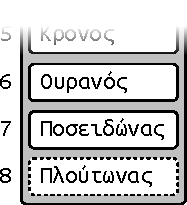
\includegraphics[scale=\scaling]{illustrations/append.pdf}
    \captionof{figure}{Η λίστα των πλανητών, μετά από την προσθήκη ενός ακόμα στοιχείου στο τέλος της.}
\end{center}}
\marginnote{Η μέθοδος \pyinline{append()} εφαρμόζεται σε μια λίστα και προσθέτει ένα νέο στοιχείο στο τέλος της. Η αντίστροφη μέθοδος είναι η \pyinline{pop()}, η οποία εφαρμόζεται σε μια λίστα κι επιστρέφει το τελευταίο στοιχείο, διαγράφοντάς το από τη λίστα.}
% κύριο πρόγραμμα: append
\pyfilesrc[firstline=13,lastline=16]{src/planets.2.py}

Παρατηρούμε ότι μπορούμε να προσθέτουμε (ή και να αφαιρούμε) στοιχεία κατά βούληση, τροποποιώντας το μέγεθος της λίστας, δηλαδή το πλήθος των στοιχείων της.

\clearpage
\section{Πες Μου Πως Σε Λένε Να Σου Πω Που Είσαι}

\begin{question}
Το παιχνίδι πρέπει να ξεκινά με ένα απλό ερώτημα. Να βρίσκει, για παράδειγμα, ο παίκτης τη θέση ενός πλανήτη στο ηλιακό σύστημα.
\end{question}

Οι ερωτήσεις προς το παίκτη δεν θα είναι πάντα ακριβώς οι ίδιες. Η δημιουργία των ερωτήσεων θα περιλαμβάνει ένα στοιχείο τυχαιότητας, συνήθως την 
επιλογή ενός από τους πλανήτες. Για τον σκοπό αυτό, θα πρέπει να εισάγουμε την κατάλληλη βιβλιοθήκη.

% import random
\pyfile[firstline=1,lastline=1]{src/planets.3.py}

Θα υλοποιούμε κάθε ερώτημα με χρήση συναρτήσεων. Έτσι θα διατηρούμε τον κώδικα μας ξεκάθαρο, αλλά και θα ξαναχρησιμοποιούμε, όπου είναι δυνατόν, τα ίδια υποπρογράμματα.

Για το πρώτο ερώτημα θα υλοποιήσουμε μια συνάρτηση η οποία δέχεται ως παράμετρο τη λίστα των πλανητών, επιλέγει από αυτή τυχαία έναν πλανήτη και, αφού εμφανίσει το όνομά του στο χρήστη, του ζητά να καθορίσει τη θέση του στο ηλιακό σύστημα. 

Ένας τρόπος να επιλεχθεί τυχαία ένας πλανήτης είναι να επιλεχθεί πρώτα ένας τυχαίος ακέραιος που θα αντιστοιχεί στη \emph{θέση} του πλανήτη μέσα στη λίστα. Η θέση αυτή θα χρησιμοποιηθεί για να προσδιορίστει και το όνομα του πλανήτη.

\marginnote[18pt]{Η συνάρτηση \pyinline{len()} επιστρέφει το πλήθος των στοιχείων της λίστας.}
% findByName part I
\pyfile[firstline=11,lastline=18]{src/planets.3.py}

\marginnote[68pt]{Μπορούμε ν' αναφερθούμε στα στοιχεία μιας λίστας με βάση τη \emph{θέση} τους σε αυτή. Η αρίθμηση των θέσεων ξεκινά από το 0. Έτσι, εδώ το πρώτο στοιχείο είναι το \pyinline{planets[0]} και αντιστοιχεί στην τιμή \pyinline{"Ερμής"}, το δεύτερο είναι το \pyinline{planets[1]} και αντιστοιχεί στην τιμή \pyinline{"Αφροδίτη"}, κ.ο.κ.}
% [comment] Αφαιρέθηκε, γιατί μπορεί να έχει προστεθεί ο Πλούτωνας: Το όγδοο και τελευταίο στοιχείο της λίστας είναι το \pyinline{planets[7]} και αντιστοιχεί στην τιμή \pyinline{"Ποδειδώνας"}.}
\marginnote{Οι θέσεις μιας λίστας αριθμούνται και αντίστροφα, ξεκινώντας από το τέλος, οπότε π.χ. στο τελευταίο στοιχείο μπορούμε να αναφερθούμε και ως \pyinline{planets[-1]}.}

Η επιλογή της τυχαίας θέσης χρειάζεται προσοχή. Οι πιθανές τιμές για την μεταβλητή \pyinline{position} κυμαίνονται ανάμεσα στο μηδέν και το πλήθος των στοιχείων της λίστας \emph{μειωμένο κατά ένα}. Αυτό συμβαίνει γιατί η αρίθμηση των θέσεων σε μια λίστα \emph{ξεκινά από το μηδέν}.

Τώρα γνωρίζουμε ότι ο πλανήτης που έχουμε επιλέξει βρίσκεται στη θέση \pyinline{position}. Το όνομα του πλανήτη βρίσκεται στην αντίστοιχη θέση μέσα στη λίστα \pyinline{planets}.

\marginnote{Για να αναφερθούμε σ' ένα στοιχείο της λίστας μπορούμε να χρησιμοποιήσουμε ανάμεσα στις αγκύλες οποιαδήποτε \emph{ακέραια έκφραση}, όπως εδώ την \pyinline{position}. Η τιμή της έκφρασης καθορίζει τη θέση του στοιχείου της λίστας στο οποίο αναφερόμαστε.}
% findByName part II
\pyfile[firstline=19,lastline=21]{src/planets.3.py}

Στη συνέχεια η συνάρτηση θα εμφανίζει την ερώτηση στον παίκτη και θα ζητάει την απάντησή του.

% findByName part III
\pyfile[firstline=22,lastline=25]{src/planets.3.py}

Η απάντηση θα πρέπει να ελεγχθεί και να εμφανίζεται είτε μήνυμα επιβράβευσης είτε η σωστή απάντηση, σε περίπτωση αποτυχίας.

% [comment] απίθανη προσθήκη: αντί για answer = position + 1, θα μπορούσαμε να γράψουμε planets[answer-1] = name. Όμως για να είναι αυτό αποδεκτό θα πρέπει πρώτα να έχουμε ελέγξει ότι 1 <= answer <= len(planets). Θα μπορούσαμε να κάνουμε τον έλεγχο με συνάρτηση. Φτιάχνουμε ούτως ή άλλως παρακάτω την reaadAnswer γι' αυτόν ακριβώς το σκοπό: την ανάγνωση ενός αριθμού εντός συγκεκριμένων ορίων. Μπορούμε να την φτιάξουμε νωρίτερα και να την ξαναχρησιμοποιήσουμε!

\marginnote[18pt]{Η παράμετρος \pyinline{sep} της \pyinline{print} καθορίζει τι θα εμφανίζεται ανάμεσα στα επιμέρους μηνύματα της \pyinline{print}. Η προκαθορισμένη τιμή της είναι η \pyinline{" "}, γι' αυτό κανονικά εμφανίζεται ένα κενό. Αν επιθυμούμε να αλλάξει αυτή η προκαθορισμένη συμπεριφορά τότε αρκεί να επανορίσουμε την \pyinline{sep}.}
% findByName part IV
\pyfile[firstline=26,lastline=33]{src/planets.3.py}

Εδώ υπάρχει και πάλι ένα λεπτό σημείο. Η θέση ενός πλανήτη στο ηλιακό σύστημα είναι κάποια τιμή από το 1 μέχρι και το πλήθος των πλανητών. Αντίθετα, η θέση του στη λίστα είναι κάποια τιμή από το 0 μέχρι και το πλήθος των πλανητών μειωμένο κατά 1. Η διαφορά αυτή οφείλεται στο γεγονός ότι οι άνθρωποι ξεκινούν την αρίθμηση θέσεων από το 1, ενώ στις λίστες η αρίθμηση ξεκινά από το 0. Κατά συνέπεια, η θέση ενός πλανήτη στο ηλιακό σύστημα είναι κατά μια μονάδα μεγαλύτερη από τη θέση του στη λίστα και γι' αυτό χρειάζεται να προσθέσουμε μια μονάδα στη μεταβλητή \pyinline{position} πριν την συγκρίνουμε με την απάντηση \pyinline{answer} του παίκτη. 

Ώρα να ξεκινήσουμε το παιχνίδι, εμφανίζοντας το πρώτο ερώτημα στον παίκτη.

\marginnote[18pt]{Το \pyinline{\n} είναι ένας ``κωδικός'' που αναπαριστά την αλλαγή γραμμής. Εδώ θέλουμε να υπάρχει μια κενή γραμμή ανάμεσα στο μήνυμα που θα εμφανιστεί και τις προηγούμενες γραμμές.}
% κύριο πρόγραμμα: κλήση της findByName
\pyfilesrc[firstline=41,lastline=43]{src/planets.3.py}

\section{Πες Μου Που Είσαι Να Σου Πω Πως Σε Λένε}

\begin{question}
Γίνεται ν' αντιστρέψουμε τώρα το ερώτημα; Να δίνεται στο χρήστη η θέση ενός πλανήτη και να ζητείται τ' όνομά του.
\end{question}

Θα υλοποιήσουμε μια ακόμα συνάρτηση, παρόμοια με την προηγούμενη, η οποία επιλέγει τυχαία έναν πλανήτη %από τη λίστα των πλανητών 
και, αφού εμφανίσει το ερώτημα στον παίκτη, ζητά και ελέγχει την απάντησή του.

% findByPosition part I
\pyfile[firstline=34,lastline=42]{src/planets.4.py}

% findByPosition part II
\pyfilesrc[firstline=43,lastline=53]{src/planets.4.py}

Τι θα γίνει όμως σε περίπτωση που ο παίκτης γράψει το όνομα του σωστού πλανήτη με κεφαλαία γράμματα ή αφήσει κενά στην απάντησή του; Παρόλο που ο παίκτης θα έχει ουσιαστικά απαντήσει σωστά, το πρόγραμμά μας θα του εμφανίζει το αντίθετο, αφού για να θεωρηθεί η απάντηση σωστή θα πρέπει να είναι πανομοιότυπη με το όνομα του πλανήτη, όπως εμφανίζεται στη λίστα των πλανητών.

Ένα μικρό και πολύ συνηθισμένο τρικ για να παρακάμψουμε αυτό το πρόβλημα είναι να συγκρίνουμε την απάντηση του παίκτη και το όνομα του σωστού πλανήτη αφού πρώτα τα μετατρέψουμε σε πεζά γράμματα, διαγράφοντας μάλιστα και τυχόν κενά που υπάρχουν στην αρχή ή στο τέλος της απάντησης.

\marginnote[18pt]{Η μέθοδος \pyinline{lower()} εφαρμόζεται σε μια αλφαριθμητική τιμή και μετατρέπει τους χαρακτήρες της σε πεζούς. Η αντίστροφη μέθοδος είναι η \pyinline{upper()}.}
\marginnote{H μέθοδος \pyinline{strip()} εφαρμόζεται σε μια αλφαριθμητική τιμή και αφαιρεί τα κενά που πιθανώς να βρίσκονται στην αρχή και το τέλος της.}
\begin{pycode}
    if answer.lower().strip() == name.lower():
\end{pycode}

Μετατρέποντας τις δύο τιμές σε μια κοινή αναπαράσταση πριν τις συγκρίνουμε μετριάζουμε σε σημαντικό βαθμό το πρόβλημα. Έχετε όμως υπόψη ότι δεν είναι και τόσο απλό να λυθεί εντελώς. Για παράδειγμα, αν ο παίκτης κάνει κάποιο ορθογραφικό λάθος ή δεν τονίσει την απάντησή του τότε και πάλι δεν θα θεωρηθεί σωστή.

Στο κύριο πρόγραμμα, μπορούμε να προσθέσουμε τη νέα ερώτηση στο παιχνίδι μας.

% κύριο πρόγραμμα: κλήση της findByPosition
\pyfilesrc[firstline=64,lastline=66]{src/planets.4.py}

\section{Η Δυσκολία Στη Ζωή Είναι Να Διαλέξεις}

\begin{question}
Όταν ο παίκτης πληκτρολογεί τις απαντήσεις του μπαίνουμε σε μπελάδες. Ας κάνουμε τις ερωτήσεις πολλαπλής επιλογής.
\end{question}

Μια ερώτηση πολλαπλής επιλογής συνοδεύεται από ένα πλήθος προκαθορισμένων απαντήσεων, από τις οποίες ο χρήστης επιλέγει εκείνη που θεωρεί σωστή. Για να παράγουμε μια ερώτηση πολλαπλής επιλογής, θα πρέπει αρχικά να γνωρίζουμε ποιες είναι οι πιθανές απαντήσεις, πόσες από αυτές θα προσφερθούν ως επιλογές στο χρήστη και, φυσικά, ποια είναι η σωστή απάντηση.

Θα μπορούσαμε λοιπόν απευθείας να υλοποιήσουμε μια συνάρτηση η οποία δέχεται τις παραπάνω παραμέτρους και παράγει μια ερώτηση πολλαπλής επιλογής.

%\begin{center}
%    \includegraphics[scale=\scaling]{illustrations/problem.pdf}
%    \captionof{figure}{Σχόλια}
%\end{center}

Ωστόσο, η παραγωγή μιας ερώτησης πολλαπλής επιλογής περιλαμβάνει συγκεκριμένα στάδια, μερικά από τα οποία δεν είναι τετριμμένα και μπορούν να υλοποιηθούν με αρκετούς διαφορετικούς τρόπους. Για τον σκοπό αυτό, κάθε στάδιο (εκτός από το τελευταίο που είναι απλό) θα υλοποιηθεί σε ξεχωριστό υποπρόγραμμα. 

% [comment] αναφορά πλεονεκτημάτων; το έχουμε κάνει ήδη % Πριν προχωρήσουμε μπορούμε να εντοπίσουμε τμήματα της συνάρτησης που θα μας χρειαστούν και σε επόμενα ερωτήματα. Με τον τρόπο αυτό θα τα κωδικοποιήσουμε σε ξεχωριστά υποπρογράμματα και θα μπορούμε να τα χρησιμοποιήσουμε ξανά, χωρίς να χρειαστεί να γράψουμε εκ νέου τον κώδικά τους.

\begin{center}
    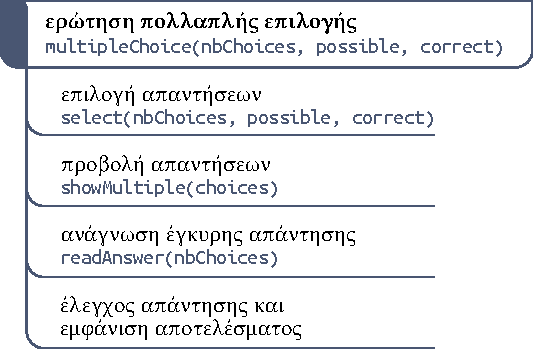
\includegraphics[scale=\scaling]{illustrations/subproblems.pdf}
    \captionof{figure}{Το πρόβλημα της παραγωγής μιας ερώτησης πολλαπλής επιλογής αναλύεται σε μικρότερα προβλήματα. Στην αναπαράσταση αυτή φαίνονται και τα υποπρογράμματα που θα δημιουργηθούν στη συνέχεια για τα προβλήματα αυτά.}
\end{center}

Για την επιλογή των πιθανών απαντήσεων θα υλοποιήσουμε μια συνάρτηση που δέχεται τη λίστα με όλες τις πιθανές απαντήσεις, καθώς και την σωστή απάντηση, επιλέγει τυχαία ένα ορισμένο πλήθος από αυτές και τις επιστρέφει σε μια λίστα, ώστε να μπορούν στη συνέχεια να εμφανιστούν στο χρήστη.

\marginnote[18pt]{Η συνάρτηση \pyinline{sample()} της βιβλιοθήκης \pyinline{random} δέχεται σαν παράμετρο μια λίστα και το πλήθος των τιμών που θα επιλεχθούν από αυτή και επιστρέφει μια νέα λίστα που περιέχει μια τυχαία επιλογή στοιχείων της πρώτης. Αν θέλουμε να επιλέξουμε τυχαία μόνο ένα στοιχείο μιας λίστας, χρησιμοποιούμε την συνάρτηση \pyinline{choice()}, της ίδιας βιβλιοθήκης.}
% select part I
\pyfile[firstline=34,lastline=43]{src/planets.5.py}

% [comment] Η χρήση της sample αφαιρεί πολλά από την "εμπειρία" του να χρησιμοποιείς λίστες, ειδικά σε αυτό το πρώιμο σημείο. 

Επειδή κάνουμε τα πρώτα μας βήματα στη διαχείριστη λιστών, χρησιμοποιήσαμε έναν ``έτοιμο'' τρόπο να επιλέξουμε ένα υποσύνολο των πιθανών απαντήσεων. Υπάρχουν και αρκετοί εναλλακτικοί τρόποι τους οποίους θα μπορέσετε να δοκιμάσετε στις ασκήσεις.

Η συνάρτηση δεν έχει ακόμα ολοκληρωθεί. Στη λίστα \pyinline{answers} των απαντήσεων που θα επιλεχθούν θα πρέπει να περιέχεται οπωσδήποτε και η σωστή απάντηση, κάτι το οποίο δεν έχουμε εξασφαλίσει. Σε περίπτωση που η σωστή απάντηση δεν περιέχεται στην \pyinline{answers}, θα πρέπει να εισαχθεί σε μια \emph{τυχαία} θέση της λίστας, \emph{αντικαθιστώντας} το στοιχείο που ήδη βρίσκεται εκεί.

\marginnote[18pt]{Ο τελεστής \pyinline{in} ελέγχει αν μια τιμή υπάρχει σε μια λίστα και επιστρέφει αντίστοιχα την τιμή \pyinline{True} ή \pyinline{False}.}
\marginnote{Χρησιμοποιώντας μια εντολή όπως η \pyinline{answers[index] = correct} \emph{τροποποιείται} ένα στοιχείο της λίστας, καθώς μια νέα τιμή αντικαθιστά την προηγούμενη. Είναι ένα βασικό χαρακτηριστικό των λιστών ότι τα στοιχεία τους μπορούν να τροποποιηθούν.}
% select part II
\pyfile[firstline=44,lastline=51]{src/planets.5.py}

Για την εμφάνιση των εναλλακτικών επιλογών θα υλοποιήσουμε μια συνάρτηση που δέχεται σαν παράμετρο τη λίστα με τις πιθανές απαντήσεις και τις εμφανίζει αριθμημένες στον παίκτη. % [comment] αφαιρέθηκε για στοιχειοθετικούς λόγους: σε μορφή πολλαπλής επιλογής. 

% [comment] αναφερόμαστε στη for ως εντολή, υπάρχει ασυνέπεια με τα προηγούμενα κεφάλαια όπου μιλούσαμε για δομές. Να διερευνηθεί μια συνεπής προσέγγιση.
% [comment] έβγαλα την περιγραφή της γενικής μορφής της for, μέχρι να δω πως την περιγράφουμε στην if και στη while.
% [comment] στις επεκτάσεις μπορεί να αναφέρει κανείς την enumerate 
\marginnote[18pt]{Η εντολή \pyinline{for} είναι μια εντολή επανάληψης που διατρέχει τα στοιχεία μιας ακολουθίας τιμών, όπως μια λίστα ή οι χαρακτήρες μιας αλφαριθμητικής τιμής, με τη σειρά με την οποία αυτά εμφανίζονται στην ακολουθία. Σε κάθε επανάληψη η τιμή του επόμενου στοιχείου της ακολουθίας ανατίθεται στη μεταβλητή απαρίθμησης που χρησιμοποιούμε στη \pyinline{for}.}
% H γενική της μορφή είναι for μεταβλητή\_απαρίθμησης in ακολουθία τιμών:
\marginnote{Όπως και στην εντολή \pyinline{while} έτσι και στη \pyinline{for} στοιχίζουμε δεξιότερα τις εντολές που περιέχονται σε αυτήν.}
% showMultiple
\pyfile[firstline=52,lastline=62]{src/planets.5.py}

Μια ακόμα συνάρτηση θα ζητάει την απάντηση του παίκτη, θα ελέγχει ότι είναι έγκυρη, δηλαδή εντός του πλήθους των πιθανών επιλογών, και θα την επιστρέφει.

% readAnswer
\pyfile[firstline=63,lastline=79]{src/planets.5.py}

\clearpage
Η τελευταία συνάρτηση που θα υλοποιήσουμε θα καλεί όλες τις προηγούμενες και θα ελέγχει αν η απάντηση που έδωσε ο παίκτης είναι σωστή ή λανθασμένη.

% multipleChoice
\pyfile[firstline=80,lastline=99]{src/planets.5.py}

Μια σημαντική παρατήρηση είναι ότι όλα τα προηγούμενα υποπρογράμματα που υλοποιήσαμε είναι τελείως ανεξάρτητα από το πρόγραμμα με τους πλανήτες. Μπορούμε να τα χρησιμοποιήσουμε για να εμφανίζουμε σε ένα πρόγραμμα ερωτήσεις τύπου πολλαπλής επιλογής ανεξάρτητα από το περιεχόμενό τους.

Πλέον μπορούμε να τροποποιήσουμε την συνάρτηση που αντιστοιχεί στο δεύτερο ερώτημα. Το αρχικό τμήμα που επιλέγει έναν τυχαίο πλανήτη και θέτει το ερώτημα στον παίκτη είναι ακριβώς το ίδιο, αλλά ακολουθείται από την κλήση της συνάρτησης για τη δημιουργία ερώτησης πολλαπλής επιλογής.

% findByPosition version II
\pyfilesrc[firstline=100,lastline=112]{src/planets.5.py}

Παρατηρήστε τις παραμέτρους με τις οποίες καλούμε την συνάρτηση \pyinline{multipleChoice()}. Καθορίζουν ότι θα εμφανιστούν στο χρήστη 4 επιλογές, ενώ η λίστα των πιθανών απαντήσεων περιλαμβάνει όλους τους πλανήτες. Ως σωστή απάντηση προσδιορίζεται βέβαια το όνομα του πλανήτη που έχει επιλεχθεί.

% [comment] Παραλείπεται για λόγους στοιχειοθεσίας: Η κλήση της συνάρτησης στο κύριο πρόγραμμα για την εμφάνιση της δεύτερης ερώτησης δεν αλλάζει καθόλου.

\section{Πες Μου Το Γείτονά Σου Να Σου Πω Ποιος Είσαι}

\begin{question}
Θα μπορούσαμε να ζητάμε από τον παίκτη να προσδιορίσει έναν πλανήτη από τους γειτονικούς του πλανήτες; 
\end{question}

Για το ερώτημα αυτό θα υλοποιήσουμε μια συνάρτηση η οποία δέχεται σαν παράμετρο τη λίστα των πλανητών, εμφανίζει τους γείτονες ενός πλανήτη και ζητά από τον παίκτη να προσδιορίσει για ποιον πλανήτη πρόκειται. Θα ξεκινήσουμε τη συνάρτηση επιλέγοντας όπως πάντα έναν τυχαίο πλανήτη.

% findByNeighbour part I
\pyfile[firstline=113,lastline=121]{src/planets.6.py}

Ο προηγούμενος πλανήτης βρίσκεται στη θέση \pyinline{position - 1} και ο επόμενος στη θέση \pyinline{position + 1}. Τί γίνεται όμως αν έχει επιλεχθεί ο πρώτος πλανήτης στη θέση 0; Τότε δεν έχει νόημα η αναφορά στη θέση \pyinline{position - 1}. Ομοίως, αν ο πλανήτης βρίσκεται στην τελευταία θέση της λίστας τότε δεν έχει νόημα η αναφορά στη θέση \pyinline{position + 1}. Το πρόγραμμά μας θα πρέπει να εξετάζει το ενδεχόμενο ο πλανήτης να βρίσκεται στα άκρα του ηλιακού συστήματος και να προσαρμόζει κατάλληλα το ερώτημα προς τον παίκτη.

% findByNeighbour part II
\pyfile[firstline=122,lastline=134]{src/planets.6.py}

% findByNeighbour part III
\pyfile[firstline=135,lastline=140]{src/planets.6.py}

Και αυτό το ερώτημα θα είναι πολλαπλής επιλογής, επομένως θα γίνει χρήση των υποπρογραμμάτων που υλοποιήσαμε προηγουμένως. Θα εμφανιστούν 4 επιλογές από τη λίστα των πλανητών, συμπεριλαμβανομένης και της σωστής.

% findByNeighbour part IV
\pyfile[firstline=141,lastline=142]{src/planets.6.py}

Πλέον μπορούμε να εμφανίσουμε το ερώτημα στον παίκτη.

% κύριο πρόγραμμα: κλήση της findByNeighbour
\pyfilesrc[firstline=156,lastline=158]{src/planets.6.py}

Παίζοντας, θα διαπιστώσουμε ότι το πρόγραμμά μας δεν λειτουργεί ακριβώς όπως θα έπρεπε. Μερικές φορές οι γειτονικοί πλανήτες εμφανίζονται τόσο στην ερώτηση όσο και στις πιθανές απαντήσεις. Θα πρέπει να διορθώσουμε τη συνάρτηση έτσι ώστε η λίστα πιθανών απαντήσεων να μην είναι ολόκληρη η λίστα των πλανητών, όπως είναι τώρα, αλλά ένα αντίγραφό της από το οποίο θα έχουμε αφαιρέσει τους γείτονες του ζητούμενου πλανήτη.

Ας ξεκινήσουμε κατασκευάζοντας το αντίγραφο, το οποίο είναι απαραίτητο προκειμένου να μην αλλοιωθεί η αρχική λίστα πλανητών.

\marginnote[-92pt]{Η μέθοδος \pyinline{copy()} εφαρμόζεται σε μια λίστα κι επιστρέφει ένα αντίγραφό της. Εδώ η δημιουργία αντιγράφου είναι απαραίτητη γιατί δεν θέλουμε να τροποποιηθεί η αρχική λίστα \pyinline{planets}. % [TODO] *** explain copy()...
\begin{center}
    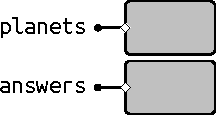
\includegraphics[scale=\scaling]{illustrations/copy.pdf}
    \captionof{figure}{Η δημιουργία αντιγράφου με την \pyinline{answers = planets.copy()} εξασφαλίζει ότι οποιαδήποτε τροποποίηση της \pyinline{answers} αφήνει την \pyinline{planets} αμετάβλητη, αφού πρόκειται για διαφορετικές λίστες.}
\end{center}
\begin{center}
    
\includegraphics[scale=\scaling]{illustrations/equal.pdf}
    \captionof{figure}{Αντίθετα, με την εντολή \pyinline{answers = planets} θα δίναμε απλά δύο ονόματα στην ίδια λίστα. Οποιαδήποτε αλλαγή στη λίστα αντικατοπτρίζεται και στα δύο ονόματα.}
\end{center}
}
\marginnote[-12pt]{Η μέθοδος \pyinline{remove()} εφαρμόζεται σε μια λίστα. Δέχεται σαν παράμετρο ένα στοιχείο της λίστας και το αφαιρεί απ' αυτή. Αν το στοιχείο δεν υπάρχει στη λίστα τότε προκύπτει σφάλμα.}
% findByNeighbour version II
\pyfile[firstline=122,lastline=123]{src/planets.7.py}

Τώρα, στα σημεία όπου προσδιορίζουμε τους γειτονικούς πλανήτες θα πρέπει να φροντίζουμε ώστε αυτοί να αφαιρούνται από τη λίστα πιθανών απαντήσεων.
% [TODO] Εδώ ο Βασιλάκης λέει να βάλουμε ολόκληρη την πολλαπλή επιλογή. Δες τι κόστος θα είχε αυτό σε χώρο κι αποφασίστε. *** πως να φαίνεται στοιχειοθετικά ότι πρόκειται για αλλαγή / επέκταση και όχι για νέο τμήμα κώδικα.

% findByNeighbour version II, corrections
\pyfile[firstline=128,lastline=130]{src/planets.7.py}

% findByNeighbour version II, corrections
\pyfile[firstline=134,lastline=136]{src/planets.7.py}

% findByNeighbour version II, corrections
\pyfile[firstline=140,lastline=144]{src/planets.7.py}

\clearpage
Οι πιθανές απαντήσεις στην ερώτηση πολλαπλής επιλογής θα πρέπει πλέον να προέρχονται από τη νέα λίστα \pyinline{answers}.
% [comment] αφαιρέθηκε για λόγους στοιχειοθεσίας: και όχι από ολόκληρη τη λίστα πλανητών.

% findByNeighbour version II, corrections
\pyfilesrc[firstline=147,lastline=148]{src/planets.7.py}

\section{Here Comes The Sun}

\begin{question}
Κάτι άλλο που θα μπορούσαμε να ζητάμε από τον παίκτη είναι να επιλέξει ποιος από τους πλανήτες που του δίνονται είναι πιο κοντά στον Ήλιο.
\end{question}

Η συνάρτηση που θα υλοποιήσουμε για το σκοπό αυτό θα ξεκινά επιλέγοντας τυχαία τον πλανήτη που θα αποτελεί την σωστή απάντηση, δηλαδή εκείνον που θα βρίσκεται πιο κοντά στον Ήλιο. Για να υπάρχουν τουλάχιστον τρεις ακόμα πλανήτες μετά τον αρχικό, η επιλογή του δεν θα γίνεται σε όλο το εύρος των στοιχείων της λίστας, αλλά σε ένα πιο περιορισμένο διάστημα.

% closestSun part I
\pyfile[firstline=149,lastline=158]{src/planets.8.py}

Για να συμπληρωθεί η ερώτηση πρέπει να δημιουργήσουμε τη λίστα των πιθανών απαντήσεων. Σε αντίθεση με προηγούμενα ερωτήματα, αυτή δεν θα προκύψει από ολόκληρη τη λίστα με τους πλανήτες, αλλά μόνο από τον επιλεγμένο πλανήτη κι αυτούς που ακολουθούν.

\marginnote[-262pt]{%
% [comment] μπορούμε να προσθέσουμε μια λεκτική περιγραφή, αν είναι απαραίτητο: Μπορούμε να \emph{τεμαχίσουμε} μια λίστα προσδιορίζοντας τις θέσεις στις οποίες ξεκινά και τερματίζεται ο τεμαχισμός. Δημιουργείται μια νέα λίστα που περιέχει μόνο το συγκεκριμένο τμήμα της αρχικής και \emph{δεν} περιλαμβάνει το στοιχείο που βρίσκεται στη θέση τερματισμού. 
\begin{center}
    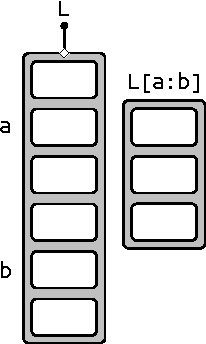
\includegraphics[scale=\scaling]{illustrations/slice.pdf}
    \captionof{figure}{Το τμήμα \pyinline{L[a:b]} είναι μια νέα λίστα που προκύπτει από τον \emph{τεμαχισμό} της λίστας~\pyinline{L}. 
    Ο τεμαχισμός σταματά \emph{πριν} το στοιχείο στη θέση~\pyinline{b}. 
    Αν παραλειφθεί η θέση εκκίνησης τότε ο τεμαχισμός ξεκινά από την αρχή της λίστας. Αν παραλειφθεί η θέση τερματισμού τότε 
    ο τεμαχισμός σταματά στο τέλος της λίστας, περιλαμβάνοντας το τελευταίο στοιχείο.}
\end{center}
}
\marginnote{%
\begin{center}
    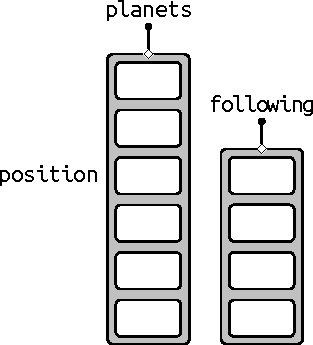
\includegraphics[scale=\scaling]{illustrations/slice-planets.pdf}
    \captionof{figure}{Η λίστα \pyinline{following} προκύπτει από τον τεμαχισμό της λίστας των πλανητών με την έκφραση
    \pyinline{planets[position : ]}.}
\end{center}
}
% closestSun part II
\pyfile[firstline=159,lastline=161]{src/planets.8.py}

Εναλλακτικά, η λίστα \pyinline{following} μπορεί να προκύψει ως εξής:

\begin{pycode}
    following = planets[position : len(planets)]
\end{pycode}

% [comment] Αυτή είναι η αρχική εκδοχή, η οποία συντομεύτηκε: Σειρά έχει η δημιουργία της λίστας των πιθανών απαντήσεων. Στο συγκεκριμένο ερώτημα υπάρχει μια ουσιώδης διαφορά σε σχέση με τα προηγούμενα. Η επιλογή των υπολοίπων απαντήσεων δεν πρέπει να γίνεται από όλη τη λίστα με τους πλανήτες, αλλά μόνο από τα στοιχεία της λίστας που βρίσκονται μετά τον επιλεγμένο πλανήτη. Επομένως, αντί να τροφοδοτήσουμε τη συνάρτηση με τη λίστα των πλανητών θα φτιάξουμε μια μικρότερη λίστα, τεμαχίζοντας την αρχική λίστα από την επόμενη θέση που βρίσκεται ο πλανήτης που επιλέξαμε μέχρι και το τέλος της.

Ας εμφανίσουμε την ερώτηση στον παίκτη.

% closestSun part III
\pyfile[firstline=162,lastline=164]{src/planets.8.py}

Ώρα για λίγο παιχνίδι ακόμα.

% κύριο πρόγραμμα: κλήση της closestSun
\pyfilesrc[firstline=181,lastline=183]{src/planets.8.py}

\section{Ο Παράταιρος}

\begin{question}
Ας ρωτήσουμε κάτι πιο περίπλοκο. Ας καλέσουμε τον παίκτη να ταξιδέψει νοερά ανάμεσα σε δύο πλανήτες και να σκεφτεί ποιους πλανήτες θα συναντήσει στη διαδρομή. Εμείς θα τον καλούμε να βρει έναν πλανήτη που \emph{δεν} θα είναι μέρος της διαδρομής.
\end{question}

% Το πρόγραμμα θα του εμφανίζει 4 πλανήτες, ένας από τους οποίους δεν θα είναι μέρος της διαδρομής και ο παίκτης θα πρέπει να τον βρει. 
Θα υλοποιήσουμε μια ακόμα συνάρτηση, στην οποία καταρχήν θα επιλέγουμε τους δύο πλανήτες που θα αποτελέσουν την αφετηρία και τον τερματισμό του ταξιδιού.

% between part I
\pyfile[firstline=165,lastline=174]{src/planets.9.py}

Παρατηρήστε ότι η αφετηρία δεν επιλέγεται απ' όλο το εύρος της λίστας, αλλά από ένα περιορισμένο διάστημα, ώστε να υπάρχουν μετά από αυτή τουλάχιστον τέσσερις πλανήτες. Ο τέταρτος από αυτούς είναι ο προορισμός της διαδρομής. 

Οι τρεις ενδιάμεσοι πλανήτες τοποθετούνται σε μια λίστα για να χρησιμοποιηθούν ως (λανθασμένες) απαντήσεις στην ερώτηση πολλαπλής επιλογής. Οι πλανήτες που δεν αποτελούν κομμάτι της διαδρομής συγκεντρώνονται επίσης σε μια λίστα, από την οποία θα επιλεχθεί τυχαία μια σωστή απάντηση.

\marginnote[-272pt]{%
\begin{center}
    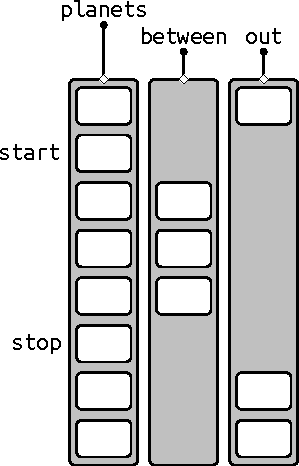
\includegraphics[scale=\scaling]{illustrations/between.pdf}
    \captionof{figure}{Η λίστα \pyinline{between} των ενδιάμεσων πλανητών και η λίστα \pyinline{out} των πλανητών που δεν αποτελούν τμήμα της διαδρομής. Και οι δύο προκύπτουν από τεμαχισμούς της \pyinline{planets} και συνενώσεις.}
\end{center}
}
\marginnote[-10pt]{Ο τελεστής \pyinline{+} χρησιμοποιείται ανάμεσα σε δύο λίστες. Το αποτέλεσμα της πράξης είναι μια νέα λίστα που περιέχει όλα τα στοιχεία των αρχικών με την ίδια σειρά.}
\marginnote{Η συνάρτηση \pyinline{choice()} της βιβλιοθήκης \pyinline{random} δέχεται σαν παράμετρο μια λίστα κι επιστρέφει ένα τυχαία επιλεγμένο στοιχείο της.}
\marginnote{Εμείς μέχρι στιγμής δεν έχουμε χρησιμοποιήσει την \pyinline{choice()} για να επιλέγουμε πλανήτες γιατί στις περισσότερες περιπτώσεις δεν χρειαζόμαστε μόνο έναν τυχαίο πλανήτη αλλά και τη θέση του μέσα στη λίστα. Έτσι, επιλέγουμε πρώτα τυχαία τη θέση ενός πλανήτη και μετά αναφερόμαστε σε αυτόν μέσω της θέσης του.}

% between part IΙ
\pyfile[firstline=175,lastline=180]{src/planets.9.py}

Πλέον είμαστε έτοιμοι να εμφανίσουμε την ερώτηση στον παίκτη μαζί με τις πιθανές επιλογές.

% between part IΙΙ
\pyfile[firstline=181,lastline=187]{src/planets.9.py}

Η λίστα των πιθανών απαντήσεων που δίνεται ως παράμετρος στην συνάρτηση \pyinline{multipleChoice}, είναι η συνένωση της λίστας \pyinline{between} των ενδιάμεσων πλανητών και μιας λίστας που αποτελείται από ένα μόνο στοιχείο: την σωστή απάντηση \pyinline{correct}.

Στη συνέχεια θα προσθέσουμε την ερώτηση στο πρόγραμμά μας.

% κύριο πρόγραμμα: κλήση της between
\pyfilesrc[firstline=207,lastline=209]{src/planets.9.py}

\section{Όλα Σε Τάξη}

\begin{question}
Ας τελειώσουμε μ' ένα ερώτημα που θα εμφανίζει στον παίκτη ανακατεμένα τα ονόματα τεσσάρων διαδοχικών πλανητών και θα του ζητά να τα βάλει σε σειρά, ξεκινώντας από τον κοντινότερο πλανήτη στον Ήλιο.
\end{question}

Η συνάρτηση που θα υλοποιήσουμε επιλέγει αρχικά τη θέση του πρώτου πλανήτη της τετράδας και δημιουργεί μια νέα λίστα που περιέχει τον πλανήτη αυτόν και τους τρεις που τον διαδέχονται.

% outOfOrder part I
\pyfile[firstline=188,lastline=197]{src/planets.10.py}

Θα δημιουργήσουμε ένα αντίγραφο της λίστας των τεσσάρων πλανητών, ώστε να τους ανακατέψουμε και να τους εμφανίσουμε στον παίκτη με τυχαία σειρά. Δεν ανακατεύουμε απευθείας την αρχική λίστα, τη χρειαζόμαστε για να υπολογίσουμε τη σωστή απάντηση.

\marginnote[18pt]{Η συνάρτηση \pyinline{shuffle()} της βιβλιοθήκης \pyinline{random} δέχεται σαν παράμετρο μια λίστα και ανακατατάσσει τις τιμές της σε τυχαίες θέσεις.}
% outOfOrder part II
\pyfile[firstline=198,lastline=201]{src/planets.10.py}

Τώρα μπορούμε να διατυπώσουμε την ερώτηση και να ζητήσουμε την απάντηση του παίκτη. Τα ονόματα των πλανητών θα εμφανίζονται αριθμημένα, ώστε ο παίκτης να γράφει τον αριθμό που αντιστοιχεί στον κάθε πλανήτη για να δώσει τη σωστή σειρά.

% outOfOrder part ΙΙΙ
\marginnote[18pt]{Η μέθοδος \pyinline{split()} εφαρμόζεται σε αλφαριθμητικές τιμές, τις οποίες χωρίζει σε επιμέρους τμήματα εκεί όπου υπάρχουν κενά και επιστρέφει μια λίστα με τα τμήματα αυτά.}
\marginnote{Εδώ, η απάντηση του χρήστη θα έχει τη μορφή \pyinline{"1 2 3 4"} και η \pyinline{split()} θα παράγει μια λίστα της μορφής \pyinline{["1", "2", "3", "4"]}.}
\pyfile[firstline=202,lastline=208]{src/planets.10.py}

\clearpage
\marginnote[18pt]{
\begin{center}
    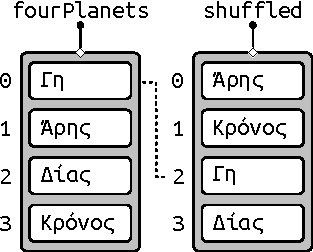
\includegraphics[scale=\scaling]{illustrations/outOfOrder-step1.pdf}%\\
    %%\vspace{100pt}
    %\mbox{}\\
    %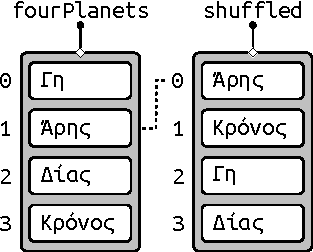
\includegraphics[scale=\scaling]{illustrations/outOfOrder-step2.pdf}
    \captionof{figure}{Ένα παράδειγμα. Η Γη είναι πρώτη στην αρχική λίστα και τρίτη στην ανακατεμένη λίστα. Άρα ο πρώτος αριθμός που πρέπει να πληκτρολογήσει ο χρήστης είναι το 3.} %Ο Άρης είναι δεύτερος στην αρχική λίστα και πρώτος στην ανακατεμένη. Άρα ο δεύτερος αριθμός που πρέπει να πληκτρολογήσει ο χρήστης είναι το 1. Ανάλογα είναι και τα δύο βήματα που απομένουν. Σε κάθε βήμα προσαρτάται στη σωστή απάντηση ακόμα ένας αριθμός.}
\end{center}
}
Για να ελέγξουμε αν η απάντηση του παίκτη είναι σωστή, χρειάζεται να κατασκευάσουμε μια λίστα αποτελούμενη από τους αριθμούς των πλανητών \emph{με τη σειρά που πρέπει να τους δώσει ο παίκτης}. 

Για να βρούμε τους αριθμούς που πρέπει να πληκτρολογήσει ο παίκτης πρέπει να διατρέξουμε την αρχική λίστα των πλανητών και για κάθε πλανήτη να υπολογίσουμε τη θέση του στην ανακατεμένη λίστα. Για παράδειγμα: ποιός είναι ο πρώτος αριθμός που πρέπει να πληκτρολογήσει ο παίκτης; Είναι ο αριθμός που έχει ο πρώτος πλανήτης της αρχικής λίστας μέσα στην ανακατεμένη λίστα.
% Εμείς διαθέτουμε τη λίστα με τους πλανήτες στην αρχική σειρά και μία με τους πλανήτες ανακατεμένους, όπως θα εμφανιστούν στον παίκτη. 
% Η λίστα με την σωστή απάντηση θα προκύψει αντιστοιχίζοντας τις θέσεις που έχουν τα στοιχεία στη λίστα \pyinline{fourPlanets}, όπου οι πλανήτες βρίσκονται σε σωστή σειρά, με τις θέσεις που έχουν στη λίστα \pyinline{shuffled}, όπου είναι ανακατεμένοι.

\marginnote{Η μέθοδος \pyinline{index()} εφαρμόζεται σε μια λίστα. Δέχεται σαν παράμετρο ένα στοιχείο της λίστας και επιστρέφει τη θέση του σε αυτή. Αν το στοιχείο δεν υπάρχει στη λίστα τότε προκύπτει \emph{σφάλμα}.}
\marginnote{Η συνάρτηση \pyinline{str()} μετατρέπει μια τιμή σε αλφαριθμητική. Εδώ είναι απαραίτητο να μετατρέψουμε τις θέσεις των πλανητών σε αλφαριθμητικές για να συγκριθούν με τις αντίστοιχες αλφαριθμητικές τιμές που θα διαβαστούν από το πληκτρολόγιο.}
% outOfOrder part ΙΙΙ
\pyfile[firstline=209,lastline=216]{src/planets.10.py}
% [comment] Χρειάζεται να γίνει κάποιο σχόλιο στο κείμενο για το +1;

Ας ελέγξουμε πλέον αν η απάντηση του παίκτη είναι σωστή.

\marginnote{Ο τελεστής \pyinline{==} μπορεί να χρησιμοποιηθεί και για να συγκριθούν δύο λίστες, στοιχείο προς στοιχείο.}
% outOfOrder part IV
\pyfile[firstline=217,lastline=222]{src/planets.10.py}

Ολοκληρώνουμε τα ερωτήματα που θα εμφανίσουμε στον παίκτη, καλώντας την συνάρτηση απ' το κύριο πρόγραμμα.

% κύριο πρόγραμμα: κλήση της outOfOrder
\pyfilesrc[firstline=245,lastline=247]{src/planets.10.py}

%%%%%%%%

%\section{Πλήρες Τελικό Πρόγραμμα}

%\pyfilesrc[firstline=1,lastline=43]{src/nim.final.py}

%%%%%%%%

\section{Τροποποιήσεις -- Επεκτάσεις}

Στο κεφάλαιο αυτό μάθαμε πολλά για τις λίστες και τους διάφορους τρόπους με τους οποίους μπορούμε να τις επεξεργαστούμε στην Python. Για να είναι ευκολότερο για εσάς να ανατρέχετε σε όλα αυτά καθώς λύνετε τις ασκήσεις, τα συγκεντρώσαμε όλα (και μερικά ακόμα) σ' ένα%
\marginnote{\href{http://pythonies.mysch.gr/cslists.pdf}{\url{pythonies.mysch.gr/cslists.pdf}}
}
\href{http://pythonies.mysch.gr/cslists.pdf}{``σκονάκι''}.

\begin{exercise}
Υλοποιήστε τη συνάρτηση \pyinline{addPluto()} έτσι ώστε να επιστρέφει την τιμή \pyinline{True} όταν η απάντηση του χρήστη περιέχεται σε μια \emph{λίστα} πιθανών καταφατικών απαντήσεων. 

\begin{note}
Μπορείτε να εφαρμόσετε τη μέθοδο \pyinline{lower()} στην απάντηση του χρήστη, οπότε η λίστα των πιθανών καταφατικών απαντήσεων θα είναι μικρότερη αφού θα πρέπει να περιέχει μόνο απαντήσεις με πεζά γράμματα.
\end{note}
\end{exercise}

\begin{exercise}
Υλοποιήστε τη συνάρτηση \pyinline{select()}, έτσι ώστε η λίστα των πιθανών απαντήσεων να κατασκευάζεται επαναληπτικά ως εξής: σε κάθε βήμα θα επιλέγεται τυχαία μια απάντηση και θα προστίθεται στη λίστα με τις πιθανές απαντήσεις μέχρι να συμπληρωθεί ο απαραίτητος αριθμός. Θα πρέπει να εξασφαλίζεται ότι η σωστή απάντηση περιλαμβάνεται στην τελική λίστα και να γίνεται ο απαραίτητος έλεγχος, ώστε να μην προστίθεται πολλές φορές ο ίδιος πλανήτης στις πιθανές απαντήσεις.

Διακρίνετε κάποιο μειονέκτημα σε μια τέτοια υλοποίηση;
\end{exercise}

\begin{exercise}
Υλοποιήστε τη συνάρτηση \pyinline{select()}, έτσι ώστε να ανακατεύεται ένα αντίγραφο της αρχικής λίστας των απαντήσεων και μετά να επιλέγεται από αυτό ένα τμήμα με τη λειτουργία του τεμαχισμού, ως λίστα πιθανών απαντήσεων. Θα πρέπει να εξασφαλίζεται ότι η σωστή απάντηση περιλαμβάνεται στην τελική λίστα.

Διακρίνετε κάποιο μειονέκτημα σε μια τέτοια υλοποίηση;
\end{exercise}

% [comment] Θα μπορούσαμε να ζητήσουμε κάτι που να περιγράφει την πραγματική υλοποίηση της sample: για κάθε δείκτη i από το 0 μέχρι το πλήθος των επιλεγόμενων στοιχείων, επιλέγουμε στην τύχη ένα στοιχείο από το i και μετά και το αντιμεταθέτουμε με το στοιχείο i. Επιστρέφεται ένα slice της λίστας μέχρι και το i.

\begin{exercise}
Μπορείτε να φτιάξετε ένα παιχνίδι με ερωτήσεις πολλαπλής επιλογής που θα αφορούν τις ημέρες της εβδομάδας, αντί για τους πλανήτες, και θα απευθύνεται σε παιδιά πρώτης δημοτικού.

\begin{note}
Mερικές ενδεικτικές ερωτήσεις: Ποιά από τις παρακάτω μέρες \emph{δεν} πηγαίνουμε σχολείο; Ποια μέρα είναι πριν ή μετά τη $x$; Αν σήμερα η μέρα είναι $x$, ποια ημέρα εννοούμε όταν λέμε ``αύριο'', ``μεθαύριο'', ``χθες'' ή ``προχθές''; Αν σήμερα η μέρα είναι $x$, τι μέρα θα είναι σε $n$ μέρες; Αν σήμερα η μέρα είναι $y$, πόσες ημέρες έχουν περάσει από τη $x$; Βάλτε στη σειρά τις παρακάτω ημέρες της εβδομάδας.
\end{note}

Εννοείται πως τα στοιχεία των ερωτήσεων που συμβολίζονται με $x$, $y$ και $n$, όπως και οι πιθανές απαντήσεις, θα επιλέγονται κάθε φορά τυχαία.
\end{exercise}

\begin{exercise}
Μπορείτε να φτιάξετε ένα παιχνίδι με παρόμοιες ερωτήσεις πολλαπλής επιλογής που θα αφορούν τους μήνες και τις εποχές, αντί για τους πλανήτες, και θα απευθύνεται σε παιδιά πρώτης και δευτέρας δημοτικού.

\begin{note}
Mερικές ενδεικτικές ερωτήσεις: Ποιός είναι ο $n$-οστός μήνας του χρόνου; Ποιος αριθμός αντιστοιχεί στον μήνα $x$; Ποιος μήνας έρχεται πριν ή μετά τον μήνα $x$; Ποιος μήνας είναι πιο κοντά στην αρχή ή στο τέλος της χρονιάς; Σε ποια εποχή ανήκει ο μήνας $x$; Ποιος μήνας δεν ανήκει στην εποχή $y$; Ποια εποχή δεν ``εκπροσωπείται'' στους παρακάτω μήνες; 
\end{note}

Εννοείται πως τα στοιχεία των ερωτήσεων που συμβολίζονται με $x$, $y$ και $n$, όπως και οι πιθανές απαντήσεις, θα επιλέγονται κάθε φορά τυχαία.

%\begin{note}
%Υπόδειξη: Για κάποιες ερωτήσεις, θα χρειαστεί να αντιστοιχίσετε τον αριθμό ενός μήνα με τον αριθμό μιας εποχής. 
%\begin{tabular}{cc}
%Μήνες & Αριθμός Εποχής & Εποχή\\
%11, 0, 1 & 0 & Χειμώνας\\
%2, 3, 4 & 1 & Άνοιξη \\
%5, 6, 7 & 2 & Καλοκαίρι\\
%8, 9, 10 & 3 & Φθινόπωρο\\
%\end{tabular}
%\end{note}
\end{exercise}

\begin{exercise}
Να τροποποιήσετε το πρόγραμμα που παίζει Πέτρα -- Ψαλίδι -- Χαρτί έτσι ώστε να χρησιμοποιεί μια λίστα που περιέχει τις λέξεις \pyinline{"Πέτρα"}, \pyinline{"Ψαλίδι"} και \pyinline{"Χαρτί"}.
Έτσι, οι (ακέραιες) επιλογές του παίκτη και του προγράμματος θα αντιστοιχίζονται άμεσα σε μια από αυτές τις λέξεις, χωρίς την ανάγκη να χρησιμοποιηθεί η \pyinline{if}.
% [comment] Να τροποποιηθεί η εκφώνηση του αρχικού προβλήματος, έτσι ώστε (α) η επιλογή του παίκτη να είναι επίσης ακεραια και (β) το πρόγραμμα να περιλαμβάνει μηνύματα: "Ο παίκτης επιλέγει ..." και "το πρόγραμμα επιλέγει ..."
\end{exercise}

\clearpage
\section{Ασκήσεις}

\begin{exercise}
Τα μπισκότα τύχης (fortune cookies) είναι μπισκότα που στο εσωτερικό τους περιέχουν μηνύματα με προβλέψεις γι' αυτόν που τα ανοίγει. Υλοποιήστε ένα πρόγραμμα που θα καλεί τον χρήστη να ανοίξει ένα τυχερό μπισκότο και στη συνέχεια θα του εμφανίζει μια τυχαία πρόβλεψη. 

\begin{note}
Μερικές ιδέες για τις προφητείες των μπισκότων: Η τύχη σου κρύβεται σε άλλο μπισκότο. Ο καλύτερος τρόπος να παραμείνεις υγιής είναι να συνεχίσεις να τρως τυχερά μπισκότα. Αποδέξου ότι κάποιες μέρες είσαι το περιστέρι και κάποιες άλλες το άγαλμα. Μαθαίνεις από τα λάθη σου... Σήμερα είναι μια μέρα που θα διδαχθείς πολλά. Η σκληρή δουλειά θα σου ανταποδώσει στο μέλλον. Η τεμπελιά θα σου ανταποδώσει άμεσα... Όλοι συμφωνούν: Είσαι ο καλύτερος!
\end{note}
\end{exercise}

\begin{exercise}
\marginnote[18pt]{Η μέθοδος \pyinline{reverse()} εφαρμόζεται σε μια λίστα κι αντιστρέφει τα στοιχεία της. Για παράδειγμα, η εντολή \pyinline{L.reverse()} αντιστρέφει τη λίστα \pyinline{L}.}
\marginnote{Ο \emph{τεμαχισμός} μπορεί επίσης να χρησιμοποιηθεί για την αντιστροφή μιας λίστας. Για παράδειγμα, η έκφραση \pyinline{L[::-1]} δημιουργεί μια νέα λίστα, που περιέχει όλα τα στοιχεία της \pyinline{L} με την αντίστροφη σειρά.}
\marginnote{Εδώ χρειάζεται ν' αντιστρέψετε μόνο ένα τμήμα της λίστας, οπότε θα χρειαστεί πρώτα να την \emph{τεμαχίσετε} και, μετά την αντιστροφή, να συνενώσετε τα τμήματά της.}
Στο παιχνίδι της αντιστροφής, εμφανίζεται στον παίκτη μια λίστα με αριθμούς κι εκείνος καλείται να τους αναδιατάξει σε αύξουσα σειρά. Το μόνο πράγμα που καθορίζει ο παίκτης σε κάθε κίνησή του είναι πόσοι αριθμοί θ' αντιστραφούν (ξεκινώντας από τ' αριστερά).

Για παράδειγμα, αν οι αριθμοί είναι:

\begin{pyterm}
2 3 4 5 1 6 7 8 9
\end{pyterm}

και ο παίκτης επιλέξει ν' αντιστρέψει τέσσερις αριθμούς, τότε οι αριθμοί θα γίνουν:

\begin{pyterm}
|\pyhighlight{5 4 3 2}| 1 6 7 8 9
\end{pyterm}

Αν στη συνέχεια ο παίκτης αντιστρέψει πέντε αριθμούς, κερδίζει!

\begin{pyterm}
|\pyhighlight{1 2 3 4 5}| 6 7 8 9
\end{pyterm}

Να κατασκευάσετε πρόγραμμα που εμφανίζει στον παίκτη μια λίστα με τους αριθμούς από το 1 μέχρι το 9 ανακατεμένους και στη συνέχεια ζητά από τον παίκτη επαναληπτικά πόσους αριθμούς να αντιστρέψει. Το παιχνίδι τελειώνει όταν ο παίκτης καταφέρει να τοποθετήσει τους αριθμούς στη σωστή σειρά ή όταν παραιτηθεί, απαντώντας ότι επιθυμεί να αντιστρέψει μηδέν αριθμούς. Αν ο παίκτης καταφέρει να ολοκληρώσει το παιχνίδι, το πρόγραμμα θα πρέπει να εμφανίζει πόσες κινήσεις χρειάστηκαν.

Όταν ολοκληρώσετε το πρόγραμμά σας, προσπαθήστε να το τροποποιήσετε έτσι ώστε οι κινήσεις να μην επιλέγονται από το χρήστη, αλλά από το πρόγραμμα, το οποίο πια θα παίζει μόνο του.
\end{exercise}

\begin{exercise}
Ο Ηλεκτρικός της Αθήνας εγκαινιάστηκε το 1869 και συνέδεε τον Πειραιά με το Θησείο. Μετά από 88 χρόνια η διαδρομή επεκτάθηκε μέχρι την Κηφισιά. Σήμερα αριθμεί 24 σταθμούς.

\marginnote[22pt]{Βρείτε τη λίστα με τους σταθμούς στο αρχείο \href{http://pythonies.mysch.gr/src/metro.py}{\url{pythonies.mysch.gr/src/metro.py}}. Αν το πρόγραμμά σας βρίσκεται στον ίδιο κατάλογο με αυτό το αρχείο μπορείτε να γράψετε \pyinline{from metro import stations} και από εκεί και πέρα θα μπορείτε να χρησιμοποιήσετε τη λίστα \pyinline{stations} με τους 24 σταθμούς.}
Υλοποιήστε ένα πρόγραμμα που θα βοηθά το χρήστη να μετακινηθεί με τον Ηλεκτρικό. Ο χρήστης θα δίνει το όνομα του σταθμού από τον οποίο θ' αναχωρήσει και το όνομα του σταθμού στον οποίο θέλει να φτάσει και το πρόγραμμα θα του εμφανίζει την κατεύθυνση που θα ακολουθήσει (προς Πειραιά ή προς Κηφισιά) και τα ονόματα όλων των ενδιάμεσων σταθμών της διαδρομής. 

\begin{note}
Ένα παράδειγμα αλληλεπίδρασης με το πρόγραμμα:

\begin{pyterm}
Δώστε σταθμό αφετηρίας
|\textbf{ΠΕΤΡΑΛΩΝΑ}|
Δώστε σταθμό προορισμού
|\textbf{ΦΑΛΗΡΟ}|
Σταθμοί από ΠΕΤΡΑΛΩΝΑ προς ΦΑΛΗΡΟ με κατεύθυνση ΠΕΙΡΑΙΑΣ
ΤΑΥΡΟΣ
ΚΑΛΛΙΘΕΑ
ΜΟΣΧΑΤΟ
\end{pyterm}
\end{note}
% [comment] Χρειάζεται έλεγχος εγκυρότητας για να μη βαρέσει καμπανάκι η index.

Μετά την εμφάνιση των πληροφοριών, το πρόγραμμα θα ρωτάει το χρήστη αν επιθυμεί πληροφορίες για κάποια άλλη διαδρομή και θα επαναλαμβάνει τη διαδικασία σε περίπτωση καταφατικής απάντησης.
\end{exercise}

\begin{exercise}
Το τρίγωνο του Pascal είναι ένας τριγωνικός μαθηματικός πίνακας με πολύ ενδιαφέρουσες ιδιότητες. Για να το κατασκευάσουμε, τοποθετούμε αρχικά στην κορυφή του τριγώνου, δηλαδή στη γραμμή 0, τον αριθμό 1. Kάθε αριθμός σε κάθε επόμενη γραμμή προκύπτει ως άθροισμα των δύο αριθμών που βρίσκονται \emph{από πάνω του}, εκτός από τον πρώτο και τον τελευταίο αριθμό κάθε γραμμής που είναι πάντα το 1.

\begin{center}
    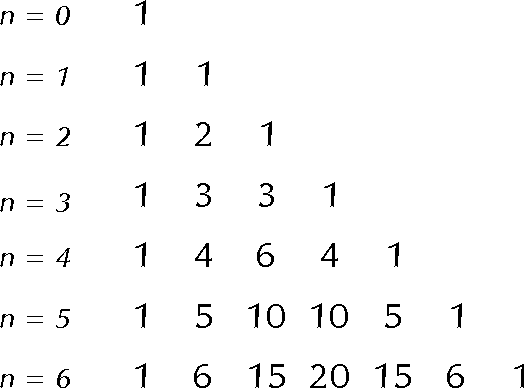
\includegraphics[scale=0.5]{illustrations/pascal-right.pdf}
    \captionof{figure}{Οι 7 πρώτες γραμμές του τριγώνου του Pascal.}
\end{center}

Από το τρίγωνο του Pascal μπορούμε να εξάγουμε τους τριγωνικούς αριθμούς και τους αριθμούς Fibonacci, να υπολογίσουμε το ανάπτυγμα πολυωνύμων ακόμα και να κατασκευάσουμε ένα φράκταλ που ονομάζεται τρίγωνο Sierpinski. 

Μια ιδιότητα του τριγώνου που θα χρησιμοποιήσουμε εμείς είναι η εξής: ο αριθμός που βρίσκεται στη γραμμή $n$ και στη στήλη $y$ αντιστοιχεί στο πλήθος των διαφορετικών τρόπων με τους οποίους μπορούμε να φέρουμε $y$ φορές κορώνα αν στρίψουμε ένα νόμισμα $n$ φορές (θυμηθείτε ότι οι γραμμές και οι στήλες αριθμούνται από το 0). Διαιρώντας αυτόν τον αριθμό με το άθροισμα των αριθμών της γραμμής $n$, το οποίο είναι $2^n$, υπολογίζουμε την πιθανότητα να φέρουμε $y$ φορές κορώνα αν στρίψουμε ένα νόμισμα $n$ φορές.

Να υλοποιήσετε ένα πρόγραμμα το οποίο διαβάζει το $n$ από το χρήστη, κατασκευάζει το τρίγωνο του Pascal μέχρι και τη γραμμή $n$ και εμφανίζει, για κάθε $y$, την πιθανότητα να φέρουμε $y$ φορές κορώνα αν στρίψουμε ένα νόμισμα $n$ φορές.
\end{exercise}

\begin{exercise}
Στο τυχερό παιχνίδι \smallcaps{Λόττο}, ο παίκτης επιλέγει έξι αριθμούς από το 1 μέχρι και το 49. Στη συνέχεια κληρώνονται έξι αριθμοί με τυχαίο τρόπο. Ανάλογα με το πλήθος των αριθμών που κατάφερε να μαντέψει ο παίκτης, έχει και τα αντίστοιχα κέρδη. 

Να υλοποιήσετε πρόγραμμα που θα ζητάει από τον χρήστη τους έξι αριθμούς της επιλογής του. Στη συνέχεια θα παράγει τους έξι τυχερούς αριθμούς που κληρώνονται. Θα πρέπει να εξασφαλίζεται ότι δεν εμφανίζεται πολλές φορές ο ίδιος αριθμός είτε στην εξάδα των τυχερών αριθμών είτε στην εξάδα των αριθμών που επιλέγει ο παίκτης.
\marginnote[2pt]{Η συνάρτηση \pyinline{sorted()} δέχεται σαν παράμετρο μια λίστα και επιστρέφει μια νέα \emph{ταξινομημένη} λίστα, χωρίς να πειράζει την αρχική. Η μέθοδος \pyinline{sort()} εφαρμόζεται σε μια λίστα και ταξινομεί τα στοιχεία της. Με τα παραπάνω θα μπορέσετε να εμφανίζετε στο χρήστη τις εξάδες των αριθμών ταξινομημένες, όπως συνηθίζεται.}
Το πρόγραμμα θα εμφανίζει στον παίκτη τους αριθμούς που επέλεξε, τους τυχερούς αριθμούς και πόσους από τους τυχερούς αριθμούς πέτυχε σωστά. 

\begin{note}
Καλό είναι να υλοποιήσετε τις επιμέρους λειτουργίες του προγράμματος με συναρτήσεις. Θα μπορούσατε να υλοποιήσετε τις εξής:
\begin{itemize}
\item \pyinline{inputNumbers()} που διαβάζει από το χρήστη 6 αριθμούς, εξασφαλίζοντας ότι βρίσκονται μεταξύ \pyinline{1} και \pyinline{49} και δεν επαναλαμβάνονται, και τους επιστρέφει σε μια λίστα.
\item \pyinline{generateNumbers()} που δημιουργεί 6 τυχαίους αριθμούς μεταξύ \pyinline{1} και \pyinline{49}, εξασφαλίζοντας ότι δεν επαναλαμβάνονται, και τους επιστρέφει σε μια λίστα.
\item \pyinline{compare()} που δέχεται σαν παραμέτρους δύο λίστες και επιστρέφει μια λίστα με τα στοιχεία που βρίσκονται και στις δύο. Εναλλακτικά, θα μπορούσε να επιστρέφει απλά το πλήθος αυτών των στοιχείων.
\end{itemize}
\end{note}
\end{exercise}

%\begin{exercise}
% Crazy Eights (που θέλει λίστα) και έχει ενδιαφέρον με τα div και mod.
%\end{exercise}

\begin{exercise}
% [comment] Αν δεν μας ενδιαφέρει η τράπουλα να ανακατεύεται και να μοιράζεται, η άσκηση θα μπορούσε να μπει και νωρίτερα, σε κεφάλαιο χωρίς λίστες. Τα χαρτιά θα παράγονται τυχαία, με μια randint.

% Πληροφορίες για τους κανόνες από το https://www.pagat.com/banking/blackjack.html
% If the dealer doesn't have a natural, he hits (takes more cards) or stands depending on the value of the hand. Contrary to the player, though, the dealer's action is completely dictated by the rules. The dealer must hit if the value of the hand is lower than 17, otherwise the dealer will stand.
Το παιχνίδι Blackjack είναι ένα παιχνίδι με χαρτιά που παίζεται από δύο παίκτες. Ένας από τους δύο κάνει τη ``μάνα'' και είναι εκείνος που διαχειρίζεται την τράπουλα. 
\marginnote[2pt]{Μπορείτε να αναπαραστήσετε την τράπουλα σαν λίστα με 52 στοιχεία. Για να κατασκευάσετε αυτή τη λίστα, μπορείτε να ξεκινήσετε με μια κενή λίστα, στην οποία θα προσθέτετε επαναληπτικά τα στοιχεία με την μέθοδο \pyinline{append()}. Εναλλακτικά, με την έκφραση \pyinline{52 * [None]}, μπορείτε να ξεκινήσετε με μια λίστα 52 στοιχείων χωρίς τιμή (αυτό είναι το \pyinline{None}) και να προσδιορίσετε επαναληπτικά την τιμή κάθε στοιχείου. Μπορείτε ακόμα και να κατασκευάσετε μια λίστα \pyinline{L}, που θα περιέχει μόνο τα 13 μοναδικά χαρτιά της τράπουλας, και μετά να κατασκευάσετε ολόκληρη την τράπουλα με την έκφραση \pyinline{L * 4}.}
Η τράπουλα περιέχει δεκατρία χαρτιά που επαναλαμβάνονται τέσσερις φορές (σύνολο 52): τα χαρτιά από 1 έως 10 και τις φιγούρες του Βαλέ, της Ντάμας και του Ρήγα. Η αξία του Βαλέ, της Ντάμας και του Ρήγα είναι 10 πόντοι, ενώ η αξία του Άσσου μπορεί να υπολογιστεί είτε ως 1 είτε ως 11, ανάλογα με το συμφέρον του παίκτη. 
%Σκοπός κάθε παίκτη είναι τα χαρτιά που θα συγκεντρώσει να έχουν το μεγαλύτερο δυνατό άθροισμα, χωρίς όμως αυτό να ξεπεράσει το 21. Αν κάποιος από τους παίκτες ξεπεράσει το 21, τότε λέμε ότι ``καίγεται'' και χάνει αυτομάτως το παιχνίδι. 

Αρχικά, %ο παίκτης ποντάρει ένα ποσό χρημάτων. Στη συνέχεια 
η τράπουλα ανακατεύεται και η ``μάνα'' με τον παίκτη παίρνουν από δύο χαρτιά ο καθένας: τα χαρτιά του παίκτη είναι ``ανοικτά'', δηλαδή φαίνεται η ένδειξή τους, ενώ η ``μάνα'' έχει ένα χαρτί ``ανοικτό'' και κρατά το άλλο ``κλειστό''. 
Η ``μάνα'' ρωτάει τον παίκτη αν επιθυμεί κι άλλο χαρτί, διαδικασία που επαναλαμβάνεται όσο ο παίκτης απαντά καταφατικά και η συνολική αξία των χαρτιών του είναι μικρότερη από 21. Στη συνέχεια, εφόσον το άθροισμα των χαρτιών του παίκτη δεν ξεπερνά το 21, η μάνα αποκαλύπτει το ``κλειστό'' της χαρτί και επαναλαμβάνει τη διαδικασία για τον εαυτό της. 
Αν κάποιος από τους δύο παίκτες ξεπεράσει το 21 τότε ``καίγεται'' και χάνει αυτομάτως. Σε διαφορετική περίπτωση, νικητής είναι εκείνος του οποίου τα χαρτιά έχουν το μεγαλύτερο άθροισμα, με τη ``μάνα'' να θεωρείται νικήτρια σε περίπτωση ισοβαθμίας.

Υλοποιήστε ένα πρόγραμμα το οποίο θα έχει το ρόλο της ``μάνας'' και θα παίζει Blackjack με αντίπαλο το χρήστη.

\begin{note}
Υπόδειξη: Όσους Άσσους κι αν έχει ένας παίκτης, μόνο ένας από αυτούς μπορεί να μετρήσει ως 11. Επομένως, το πρόγραμμά σας θα πρέπει να ελέγχει το πολύ δύο αθροίσματα, το κανονικό άθροισμα των χαρτιών και, στην περίπτωση που υπάρχει τουλάχιστον ένας Άσσος, το λεγόμενο ``μαλακό'' άθροισμα, στο οποίο ο Άσσος μετράει ως 11.
\end{note}
\end{exercise}

%%%%%%%%

\section*{}
\vspace{2\parskip}
\hrulefill

\begin{theory}{Δομές Δεδομένων και Λίστες}
Οι λίστες, δομές απλές κι ευέλικτες, έχουν βαρύνουσα σημασία στην ιστορία της Πληροφορικής. Η δεύτερη γλώσσα προγραμματισμού που αναπτύχθηκε, η LISP του John McCarthy, βασίζεται στις λίστες. Η Logo, με την σειρά της, μια ιστορική εκπαιδευτική γλώσσα προγραμματισμού, βασίζεται κυρίως στη LISP.

Οι λίστες είναι ένα παράδειγμα \emph{οργάνωσης} των δεδομένων μας, έτσι ώστε να αποτελούν μια ενιαία συλλογή με συγκεκριμένη \emph{δομή}. Υπάρχουν αναρίθμητοι τρόποι να οργανώσουμε τα δεδομένα μας, γι' αυτό και υπάρχουν και πάρα πολλές δομές δεδομένων. Ακόμα και οι πιο θεμελιώδεις έχουν εξωτικά ονόματα όπως \emph{στοίβες}, \emph{ουρές}, \emph{δέντρα}, \emph{σωροί} ή \emph{γράφοι}. Ο τρόπος οργάνωσης καθορίζει πόσο εύκολο είναι να επεξεργαστούμε τα δεδομένα μας με συγκεκριμένο τρόπο. Γι' αυτό και επιλέγουμε τη δομή που θα χρησιμοποιήσουμε κάθε φορά ανάλογα με τον συγκεκριμένο τρόπο που θέλουμε να επεξεργαστούμε τα δεδομένα μας, στα πλαίσια ενός συγκεκριμένου προβλήματος.

Μέχρι να αντιμετωπίσει κανείς στοιχειωδώς περίπλοκα προβλήματα είναι δύσκολο να διακρίνει \emph{γιατί} χρειάζεται να οργανωθούν τα δεδομένα -- οι μεμονωμένες μεταβλητές φαίνονται υπεραρκετές, αλλά δεν είναι. Αν είστε άνθρωποι με περιπετειώδες πνεύμα, μπορείτε να επιχειρήσετε να υλοποιήσετε το παιχνίδι αυτού του κεφαλαίου χωρίς να χρησιμοποιήσετε λίστες.
\end{theory}

\begin{theory}{Αρίθμηση από το Μηδέν}
Υπάρχουν δύο ειδών άνθρωποι στον κόσμο: (1) αυτοί που ξεκινούν την αρίθμηση από το ένα και (1) αυτοί που ξεκινούν την αρίθμηση από το μηδέν. Αν πιάσατε το αστειάκι, έχετε καταλάβει αυτό το λεπτό σημείο του κεφαλαίου. Η χρήση της αρίθμησης από το μηδέν ξεκίνησε τη δεκαετία του '60 από ανάγκη, για καθαρά τεχνικούς λόγους και είναι αλήθεια ότι σε εκείνους που την συναντούν για πρώτη φορά φαίνεται από άβολη έως παρανοϊκή. Ωστόσο, έχει και σημαντικά πλεονεκτήματα. Ο ιδιόρυθμος Edsger Dijkstra, ένας από τους ανθρώπους που συνέβαλαν καθοριστικά στην καθιέρωση της Πληροφορικής ως επιστήμη, έγραψε το 1982 τρεις ολόκληρες (χειρόγραφες) σελίδες με τίτλο ``Γιατί η αρίθμηση πρέπει να ξεκινά από το μηδέν''. Τώρα, η αρίθμηση από το μηδέν είναι πια από τα πολύ χαρακτηριστικά ιδιώματα της Πληροφορικής. Στο παιδικό βιβλίο ``Lauren Ipsum'' του Carlos Bueno, η αρίθμηση των κεφαλαίων ξεκινά από το μηδέν και η ηρωίδα, καθώς αρχίζει την περιπέτειά της, συναντά μια πινακίδα όπου το πρώτο μίλι της διαδρομής είναι φυσικά... το μηδενικό.
\end{theory}

%\marginnote[-100pt]{
\marginnote[18pt]{
\begin{center}
    
\includegraphics[scale=0.35]{images/mile-0.png}
    \captionof{figure}{Από το Κεφάλαιο 0 του Lauren Ipsum.}
\end{center}}

%“Ah, here we are,” he said. “Route One, Mile Zero.”
%“I’ve never seen a Mile ZERO,” said Laurie.
%“Everything has to start somewhere. It may not look like much, but this is a very special place. You might even say it’s the starting point of the whole System.”
%“What comes after Mile Zero?”
%“Mile One, of course. And right after that is the town of Bach. Are you ready?”

\hrulefill

%%%%%%%%%

\end{document}

\begin{exercise}
% προτείνω να μπει σε άλλο κεφάλαιο
Φανταστείτε ότι ενώ κάνετε μια βόλτα αμέριμνοι με τους φίλους σας, ξαφνικά περικυκλώνεστε από μια συμμορία κακοποιών στοιχείων, που δεν φαίνεται να έχουν και τις καλύτερες διαθέσεις απέναντί σας! Για καλή σας τύχη, ο αρχηγός της συμμορίας είναι φανατικός λάτρης των γρίφων και των αλγοριθμικών παζλ, οπότε δίνει μια τελευταία ευκαιρία σε έναν από εσάς να επιζήσει. Σας ανακοινώνει ότι θα σταθείτε όλοι στη σειρά και οι άντρες του θα αρχίσουν να σκοτώνουν τα άτομα της σειράς ανά δυο. 
Η διαδικασία θα επαναλαμβάνεται κάθε φορά με τα άτομα που απομένουν μέχρι να μείνει μόνο ένας ζωντανός! Ποια θέση θα επιλέξετε στη σειρά για να μείνετε ζωντανός; Κάπως έτσι πρέπει να αισθάνθηκε ο εβραίος ιστορικός Ιώσηπος, τον 1\textsuperscript{ο} αιώνα μ.Χ. όταν εκείνος και οι άντρες του έπεσαν στα χέρια Ρωμαίων στρατιωτών.

Σκοπός είναι να υλοποιήσετε ένα παιχνίδι – προσομοίωση του προβλήματος του Ιωσήπου. Το πρόγραμμά σας θα ανακοινώνει στον παίκτη το συνολικό αριθμό των ατόμων που θα σχηματίσουν σειρά και το «βηματισμό» με τον οποίο θα σκοτώνονται τα άτομα και στη συνέχεια θα τον ρωτά σε ποια θέση θέλει να σταθεί. Τέλος θα του εμφανίζει αν η επιλογή του ήταν σωστή, δηλαδή αν κατάφερε να επιβιώσει ή αν είναι πολύ αργά για να ξαναπροσπαθήσει!
% [comment]: γιατί χρειάζεται λίστα;
% [comment]: από ποιον ξεκινάνε να σκοτώνουν, από τον πρώτο;
% [comment]: τι γίνεται όταν το βήμα είναι k κι απομένουν λιγότεροι από k;
\end{exercise}

\begin{exercise}
Το παιχνίδι χαρτιών Πόλεμος (War) παίζεται ανάμεσα σε δύο παίκτες. 
Η τράπουλα αποτελείται από δεκατρία χαρτιά που επαναλαμβάνονται τέσσερις φορές (σύνολο 52): τα χαρτιά από 1 έως 10 και τις φιγούρες του Βαλέ, της Ντάμας και του Ρήγα. Στον Πόλεμο, το χαρτί με την μεγαλύτερη αξία είναι ο Άσσος (το 1) και ακολουθούν σε φθίνουσα σειρά ο Ρήγας, η Ντάμα, ο Βαλές, το 10, το 9, κλπ. μέχρι το 2.

Αρχικά, η τράπουλα ανακατεύεται και οι παίκτες μοιράζονται τα χαρτιά της, παίρνοντας ο καθένας από 26 και τοποθετώντας τα σε στοίβα ``κλειστά'', δηλαδή γυρισμένα με τη φιγούρα προς τα κάτω. 
Σε κάθε γύρο, ο κάθε παίκτης τραβάει το κορυφαίο χαρτί από τη στοίβα του και το τοποθετεί ``ανοικτό'' στο τραπέζι. Ο παίκτης με το χαρτί μεγαλύτερης αξίας παίρνει και τα δύο χαρτιά από το τραπέζι και τα τοποθετεί \emph{στον πάτο} της στοίβας του. Στην περίπτωση που οι δύο παίκτες τραβήξουν χαρτιά ίσης αξίας τότε ξεκινάει πόλεμος μεταξύ τους. Τραβάει ο καθένας άλλα δύο χαρτιά από την στοίβα τους, κρατούν το ένα ``κλειστό'' και συγκρίνουν το άλλο. Ο παίκτης με το χαρτί μεγαλύτερης αξίας παίρνει και τα έξι χαρτιά από το τραπέζι και τα τοποθετεί \emph{στον πάτο} της στοίβας του, αλλιώς ο πόλεμος συνεχίζεται.
Νικητής του παιχνιδιού θεωρείται ο παίκτης που θα μαζέψει όλα τα χαρτιά της τράπουλας.

% [comment][changed] Αποφεύγω πολύ τη φράση "με αντίπαλο τον υπολογιστή" γιατί δημιουργεί παρανοήσεις. Το ίδιο το πρόγραμμα είναι ο αντίπαλος.
%Υλοποιήστε ένα πρόγραμμα στο οποίο ο παίκτης θα παίζει Πόλεμο με αντίπαλο τον υπολογιστή.

Υλοποιήστε ένα πρόγραμμα το οποίο θα παίζει Πόλεμο με αντίπαλο το χρήστη.

\begin{note}
Σημείωση: Όταν ο νικητής ενός γύρου μαζεύει από το τραπέζι τα χαρτιά που κέρδισε και τα τοποθετεί στον πάτο της στοίβας του, δεν θα πρέπει να το κάνει πάντα με την ίδια σειρά, π.χ. πρώτα τα δικά του και μετά του αντιπάλου, αλλά με \emph{τυχαία} σειρά. Σε διαφορετική περίπτωση, το πιθανότερο είναι πως το παιχνίδι δεν θα τελειώσει ποτέ.
\end{note}

% [comment] Δεν έχουμε καμία καθοδήγηση ως προς τις αναπαραστάσεις ή τις συναρτήσεις που θα χρησιμοποιηθούν. Να τους καθοδηγήσουμε πως θα αναπαραστήσουν την τράπουλα και πως θα μοιράσουν τα χαρτιά με slices;
\end{exercise}

